\documentclass[12pt]{report}
\pagestyle{plain}

%\usepackage{subfigure}
\usepackage{cancel}
\usepackage{setspace}
\usepackage[sorting = none]{biblatex}
\usepackage{amssymb,graphicx,color}
\usepackage{amsfonts}
\usepackage{latexsym}
\usepackage{a4wide}
\usepackage{amsmath}
\usepackage{csvsimple}
\usepackage{booktabs}
\usepackage[utf8]{inputenc}
\usepackage{todonotes}
\usepackage{bigints}
\usepackage{hyperref}
\usepackage{subcaption}

\allowdisplaybreaks

\hypersetup {
    hidelinks
}

\addbibresource{references.bib}

\newtheorem{theorem}{THEOREM}
\newtheorem{lemma}[theorem]{LEMMA}
\newtheorem{corollary}[theorem]{COROLLARY}
\newtheorem{proposition}[theorem]{PROPOSITION}
\newtheorem{remark}[theorem]{REMARK}
\newtheorem{definition}[theorem]{DEFINITION}
\newtheorem{fact}[theorem]{FACT}

\newtheorem{problem}[theorem]{PROBLEM}
\newtheorem{exercise}[theorem]{EXERCISE}
\def \set#1{\{#1\} }

\newenvironment{proof}{
PROOF:
\begin{quotation}}{
$\Box$ \end{quotation}}


\DeclareMathOperator{\EX}{\mathbb{E}}% expected value
\DeclareMathOperator{\VAR}{\mathbb{V}}% expected value
\DeclareMathOperator*{\argmin}{arg\,min}
\DeclareMathOperator*{\argmax}{arg\,max}

\newcommand{\bs}{\boldsymbol}
\newcommand{\tb}{\textbf}
\newcommand{\pc}[2]{p(#1 \mid #2)}
\newcommand{\mc}[1]{\mathcal{#1}}
\newcommand{\mb}[1]{\mathbb{#1}}
\newcommand{\half}{\frac{1}{2}}
\newcommand{\E}{\mathbb{E}}
\newcommand{\inv}[1]{#1^{-1}}
\newcommand{\sumlim}[3]{\sum\limits_{#1 = #2}^{#3}}
\newcommand{\suml}[1]{\sum\limits_{#1}}
\newcommand{\prodlim}[3]{\prod\limits_{#1 = #2}^{#3}}
\newcommand{\prodl}[1]{\prod\limits_{#1}}
\newcommand{\ub}{\underbrace}
\newcommand{\intlim}[2]{\int\limits_{#1}^{#2}}
\newcommand{\diff}[1]{\frac{d}{d#1}}
\newcommand{\prl}{\partial}
\newcommand{\ol}{\overline}
\newcommand{\argminl}[1]{\argmin\limits_{#1}^{}}
\newcommand{\argmaxl}[1]{\argmax\limits_{#1}^{}}
\newcommand{\comb}[2]{\begin{pmatrix}#1 \\ #2\end{pmatrix}}

\renewcommand{\P}{\mathbb{P}}
\renewcommand{\bs}{\boldsymbol}

%%%%%%%%%%%%%%%%%%%%%%%%%%

\title{  	{ 
\includegraphics[scale=.5]{ucl_logo.png}}\\
{{\Huge Inference In Latent Random Geometric Graphs}}\\
		}
\date{Submission date: $11^\text{th}$ of September 2020}
\author{R\u{a}zvan - Dumitru Meriniuc\thanks{
{\bf Disclaimer:}
This report is submitted as part requirement for the Machine Learning MSc at UCL. It is
substantially the result of my own work except where explicitly indicated in the text.
The report may be freely copied and distributed provided the source is explicitly acknowledged.}
\\ \\
Machine Learning MSc\\ \\
Peter Orbanz}

\begin{filecontents*}{test_spherical_gaussian_m1.csv}
Original $\sigma$,Original Edges,Model Edges,TVD $d_k$,TVD $\chi_k$,TVD $\gamma_k$,Inferred $\sigma$ 
0.1,43124.9 ± 106.419,42813.55 ± 155.108,0.222 ± 0.043,0.183 ± 0.066,0.007 ± 0.003,0.109
0.4,27345.25 ± 438.729,29378.55 ± 601.806,0.408 ± 0.029,0.188 ± 0.05,0.045 ± 0.011,0.358
0.7,15331.75 ± 593.006,20350.2 ± 854.684,0.547 ± 0.032,0.399 ± 0.063,0.112 ± 0.014,0.543
1.0,8959.2 ± 509.642,15350.25 ± 955.845,0.619 ± 0.04,0.551 ± 0.066,0.148 ± 0.016,0.694
1.3,5768.0 ± 354.239,12305.05 ± 577.811,0.665 ± 0.038,0.636 ± 0.06,0.303 ± 0.027,0.816
1.6,4064.95 ± 205.598,10115.4 ± 446.654,0.685 ± 0.024,0.67 ± 0.022,0.424 ± 0.02,0.916
1.9,2948.55 ± 255.48,8916.75 ± 742.017,0.729 ± 0.034,0.719 ± 0.058,0.51 ± 0.03,1.012
2.2,2250.65 ± 139.114,7842.2 ± 448.166,0.756 ± 0.026,0.744 ± 0.039,0.554 ± 0.018,1.094
2.5,1724.5 ± 102.614,6669.15 ± 304.363,0.763 ± 0.017,0.757 ± 0.031,0.597 ± 0.026,1.178
2.8,1378.75 ± 101.247,6270.95 ± 410.756,0.789 ± 0.03,0.791 ± 0.038,0.666 ± 0.028,1.251
3.1,1132.65 ± 90.562,5612.65 ± 301.734,0.798 ± 0.03,0.799 ± 0.026,0.702 ± 0.027,1.316
3.4,942.85 ± 54.53,5319.45 ± 362.87,0.812 ± 0.016,0.819 ± 0.027,0.731 ± 0.013,1.377
\end{filecontents*}

\begin{filecontents*}{test_spherical_multivariate_t_m1.csv}
Original $\sigma$,Original Edges,Model Edges,TVD $d_k$,TVD $\chi_k$,TVD $\gamma_k$,Inferred $\sigma$
0.1,42829.3 ± 143.05,42488.15 ± 220.543,0.227 ± 0.041,0.2 ± 0.062,0.008 ± 0.003,0.116
0.4,26261.0 ± 713.03,28666.35 ± 768.418,0.431 ± 0.035,0.182 ± 0.05,0.054 ± 0.012,0.373
0.7,14390.9 ± 667.362,20057.45 ± 1083.909,0.559 ± 0.037,0.412 ± 0.078,0.126 ± 0.018,0.561
1.0,8333.4 ± 436.009,14479.5 ± 652.509,0.604 ± 0.035,0.505 ± 0.066,0.175 ± 0.019,0.713
1.3,5385.9 ± 218.601,11976.2 ± 793.809,0.667 ± 0.038,0.63 ± 0.065,0.338 ± 0.02,0.835
1.6,3814.3 ± 263.402,9945.45 ± 462.539,0.696 ± 0.028,0.665 ± 0.061,0.458 ± 0.024,0.935
1.9,2739.45 ± 134.691,8670.4 ± 533.589,0.73 ± 0.027,0.718 ± 0.039,0.53 ± 0.02,1.034
2.2,2063.25 ± 189.725,7486.75 ± 595.039,0.751 ± 0.026,0.757 ± 0.033,0.558 ± 0.023,1.123
2.5,1674.75 ± 123.0,6766.5 ± 444.277,0.752 ± 0.031,0.757 ± 0.026,0.62 ± 0.021,1.188
2.8,1254.85 ± 85.145,5946.75 ± 322.501,0.788 ± 0.024,0.797 ± 0.023,0.682 ± 0.017,1.282
3.1,1067.4 ± 75.707,5581.9 ± 403.393,0.794 ± 0.031,0.787 ± 0.035,0.711 ± 0.02,1.336
3.4,888.45 ± 68.564,5035.3 ± 320.16,0.805 ± 0.032,0.799 ± 0.029,0.745 ± 0.024,1.398
\end{filecontents*}

\begin{filecontents*}{test_ms.csv}
$n$,Original Edges,Model Edges,TVD $d_k$,TVD $\chi_k$,TVD $\gamma_k$,Inferred $\sigma$
2,9003.15 ± 441.038,15240.7 ± 690.233,0.609 ± 0.034,0.521 ± 0.067,0.143 ± 0.014,0.692
4,1821.05 ± 138.203,4380.55 ± 259.205,0.512 ± 0.037,0.503 ± 0.069,0.411 ± 0.023,0.74
6,348.9 ± 33.139,1120.65 ± 126.861,0.47 ± 0.031,0.359 ± 0.064,0.562 ± 0.047,0.78
8,72.4 ± 10.2,316.35 ± 37.373,0.395 ± 0.037,0.118 ± 0.06,0.141 ± 0.034,0.783
10,14.55 ± 4.748,110.6 ± 16.951,0.338 ± 0.048,0.044 ± 0.037,0.011 ± 0.004,0.762
12,2.3 ± 1.52,43.9 ± 8.831,0.206 ± 0.032,0.083 ± 0.177,0.002 ± 0.001,0.737
\end{filecontents*}

\begin{filecontents*}{test_close.csv}
Original Edges,Model Edges,TVD $d_k$,TVD $\chi_k$,TVD $\gamma_k$,Inferred $\sigma$
5082.8 ± 265.968,11342.1 ± 550.784,0.673 ± 0.037,0.623 ± 0.059,0.38 ± 0.023,0.852
\end{filecontents*}

\begin{filecontents*}{test_far.csv}
Original Edges,Model Edges,TVD $d_k$,TVD $\chi_k$,TVD $\gamma_k$,Inferred $\sigma$
4104.45 ± 268.468,10177.5 ± 837.822,0.661 ± 0.033,0.579 ± 0.06,0.523 ± 0.018,0.914
\end{filecontents*}

\begin{filecontents*}{test_skewed_g.csv}
Original Edges,Model Edges,TVD $d_k$,TVD $\chi_k$,TVD $\gamma_k$,Inferred $\sigma$
8338.75 ± 394.827,14763.45 ± 686.497,0.648 ± 0.038,0.503 ± 0.065,0.305 ± 0.02,0.713
\end{filecontents*}

\begin{filecontents*}{test_skewed_t.csv}
Original Edges,Model Edges,TVD $d_k$,TVD $\chi_k$,TVD $\gamma_k$,Inferred $\sigma$
7653.9 ± 318.023,14312.55 ± 838.109,0.659 ± 0.043,0.528 ± 0.072,0.341 ± 0.019,0.737
\end{filecontents*}

\doublespacing

\begin{document}
 
\maketitle
\begin{abstract}
    The graph is a ubiquitous data structure, arising in numerous real-world scenarios, ranging from social networks to drug design. While relatively simple, it is difficult to exploit it in the context of machine learning, which prompts one to find ways of encoding it in a geometric space with a well-defined metric. Our work aims to study the feasibility of treating the embeddings of the nodes of a graph as latent variables, in the context of random geometric graphs (RGG) and Bayesian statistics. By placing a prior on the embeddings and drawing an edge between two points randomly, based on the distance between them, we intend to approximate the posterior of the embeddings, given the graph, which would allow us to better describe the geometry capturing the properties of the graph.

\end{abstract}
\tableofcontents
\setcounter{page}{1}


\chapter{Introduction}
Learning representations of symbolic data such as graphs, multi-relational data and text is an essential paradigm in artificial intelligence and machine learning. For example, in the field of Natural Language Processing, embeddings of words, such as \texttt{WORD2VEC}~\parencite{word2vec}, \texttt{GLOVE}~\parencite{glove} and \texttt{FASTTEXT}~\parencite{fasttext} have proven crucial for advancing the field, leading to the excellent results in tasks such as machine translation and sentiment analysis. Similarly, embeddings of graphs, such as \texttt{NODE2VEC}~\parencite{node2vec}, \texttt{DEEPWALK}~\parencite{deepwalk} and latent space embeddings~\parencite{hoff2002latent}. \texttt{RESCAL}~\parencite{rescal}, \texttt{TRANSE}~\parencite{transe} and Universal Schema~\parencite{universalschema} are examples of embeddings of multi-relational data that are used in knowledge graphs and information extraction. \\

The graph is a ubiquitous data structure, which arises in numerous real-world scenarios, ranging from social networks~\parencite{socialnetwork} to drug design~\parencite{graphprotein}. Its relative simplicity allows one to attach a myriad of semantics to the nodes and edges, hence its prevalence. However, its format limits the scope of machine learning techniques one can use on such data, but embedding its vertices in a geometry, be it euclidean or with a non-zero curvature, allows us to extend the range of methods we can use while modelling the data. This idea arises naturally, as many networks coming from physical considerations are governed by an underlying geometry, such as the road network in a country. Moreover, it enables us to work in a space which is endowed with more modelling approaches and ties well into the concept of two similar entities being \textit{close} to each other. \\

We are going to focus on data given as a simple homogeneous graph, i.e unweighted, undirected graph that contains no self-loops and no multiple edges~\parencite{simplegraphdef}. The homogeneity refers to the edges representing the same concept. Mathematically, we define it as a pair $G = (V, E)$, where $V$ is the set of vertices, also called nodes, and $E$ is the set of edges. We will represent the vertices as consecutive natural numbers, so $V = \{1,\,2,\,\dots\,N\}$, and the edges as unordered pairs $\{i,\, j\}$, $i \neq j$, $i,\,j \in V$. Such a graph can be completely defined by its adjacency matrix, $A$, $A_{ij} = 1$ if $\{i,\,j\} \in E$ and 0 otherwise, as we are working with unweighted edges, so we are interested whether an edge exists or not. Since the graph is undirected, $A_{ij} = A_{ji}$. \\

The aim of this project is to study the feasibility of performing inference on the latent geometric embeddings, in a Bayesian setting. The literature generally focuses on empirical embeddings, targeting the individual nodes, while we are more interested in their underlying distribution. A random geometric graph (RGG) is usually generated by sampling points from some space, which represent the nodes, and connecting each pair by an edge if the distance between them is less than some fixed threshold. In order to avoid this step function and the extra hyperparameter, we generate an edge stochastically, again relying on the distance between the points. The closer two points are, the greater the chance of them being connected. \\

In the literature, embeddings of nodes~\parencite{word2vec, line, watch} , edges~\parencite{edge2vec, edgeembedd} and even whole subgraphs~\parencite{subrank, sub2vec} have been studied. We are going to focus on embedding of nodes only. Random geometric graphs are generally studied from a graph theoretical or algorithmic point of view. We aim, however, to describe in probabilistic terms the distribution of the embeddings and perform inference, which has not been studied so far, to our knowledge.

\chapter{Background And Related Work}

\section{Bayesian Statistics And Variational Inference}

We are going to work in the framework of Bayesian statistics, which relies on the Bayesian interpretation of probabilities, where the probability conveys the degree of belief in an event, which may rely on prior knowledge about the event, whether it is a personal belief or based on results of previous experiments. This is in contrast to the frequentist interpretation, which views probability as the limit of the relative frequency of an event after a large number of trials~\parencite{frequentist}. \\

The cornerstone of Bayesian statistics is Bayes' formula. If $X$ is some data generated by a process with parameter $\theta$, then

\begin{definition}[Bayes' Formula, Posterior, Likelihood, Prior, Evidence]
\label{eq:bayesdef}
\begin{equation*}
    \mb{P}(\theta \mid X) = \frac{\mb{P}(X \mid \theta)\mb{P}(\theta)}{\mb{P}(X)}
\end{equation*}
\begin{enumerate}
    \item The \textbf{posterior} distribution, $\mathbb{P}(\theta \mid X)$, represents our updated belief about the parameter $\theta$ after observing the data $X$.
    \item The \textbf{likelihood} distribution, $\mathbb{P}(X \mid \theta)$, denotes the probability of the data being generated by the given the parameter $\theta$.
    \item The \textbf{prior} distribution, $\mathbb{P}(\theta)$, quantifies our assumption about the parameter $\theta$.
    \item The \textbf{evidence} distribution, $\mathbb{P}(X)$, represents the probability of the data occurring, which is computed by marginalising out the parameter $\theta$.
\end{enumerate}
\end{definition}

The central Bayesian principle consists of placing a probability over the parameters, thus giving rise to the prior. It is asymptotically equivalent to the frequentist method, the parameter converging to the true one~\parencite{bayesconsistency}, but the downside is that there is no mathematical decision theory one can rely on when choosing the prior. It is totally up to the practitioner, which allows us to insert our belief into the model, thus forcing us to be honest about the assumptions we make regarding the data and learning process. \\

Statistical inference is the process of using data analysis to deduce properties of an underlying probability distribution~\parencite{statinference}. For example, if we model some data according to a Gaussian distribution with a known variance, we can look at the data and infer what the mean is, and then use it to make predictions on new input points. When predicting, we could work with the parameter for which the data is most likely to occur, an estimate known as MAP (Maximum a posteriori), or average over the parameters in a Bayesian setting, by marginalisation, such that each element of the average has a weight represented by the posterior:

\newpage
\begin{align}
    \mathbb{P}(\textbf{X*} \mid \textbf{X}) &= \int_{\Theta} \mathbb{P}(\textbf{X*}, \theta \mid \textbf{X}) d\theta\\
    &= \int_{\Theta} \mathbb{P}(\textbf{X*} \mid \theta, \textbf{X}) \mathbb{P}(\theta \mid \textbf{X}) d\theta \\ 
    &= \int_{\Theta} \mathbb{P}(\textbf{X*} \mid \theta) \mathbb{P}(\theta \mid \textbf{X}) d\theta \label{predict}\\
    &= \E_{\P(\theta \mid \bs{X})}[\P(\bs{X^*} \mid \theta)], \notag
\end{align}

\noindent
where $\textbf{X}$ is the observed data, $\textbf{X*}$ are the points for which we are trying to predict a quantity of interest, $\Theta$ is the parameter space and $\theta$ is an arbitrary parameter. $\P(\textbf{X*} \mid \theta, \textbf{X})$ becomes $\P(\textbf{X*} \mid \theta)$ because the model is fully specified given the parameters, the known points $\bs{X}$ adding no information. \\

\noindent
This integral requires a closed form of the posterior, which is often intractable because we cannot calculate the evidence present in the denominator in \textbf{Definition 1}, $\P(\bs{X})$. Even if it can be calculated, the posterior is not usually the probability density function a known distribution, which would make it more difficult to study and use. A possible solution would be to approximate it with the average $\frac{1}{N}\sum\limits_{i = 1}^N \P(\bs{X^*} \mid \theta_i)$, where $\{\theta_i\}_{i = 1}^N$ are the samples from $\P(\theta \mid \bs{X})$. The most popular class of sampling algorithms is Markov Chain Monte Carlo (MCMC)~\parencite{mcmc}. For example, the Metropolis -- Hastings algorithm~\parencite{metropolis} allows us to circumvent the evidence, which cancels out. One of the drawbacks of this method is that it is non-deterministic and, in addition, we would not be able to measure how good our approximation is. Furthermore, there is the problem of choosing the hyperparameters, parameters of the model that are not governed by a prior, as they are just scalars whose value we need to determine. The classical approach aims to maximise the probability of the observed data, $\P(\bs{X})$, which is the term that generates the intractable integral preventing us from calculating the posterior in the first place. We could again employ sampling to address this issue, adding an extra layer of randomness to our implementation, which is undesirable. The technique we are about to present deals with the approximation of the posterior with a new variational distribution, offering a measure of \textit{distance} between the distributions, thus allowing us to determine how good our approximation is, which means that there is some quantity that tells us if we are working in the right direction. The setting of this approach offers a lower bound of the evidence as a by-product, while we are making the approximation better, which is where the beauty of this method lies. While it does not provide a hard maximum for the evidence, we get the next best thing, a lower bound. \\

\noindent
The measure between distributions is called the Kullback -- Leibler (KL) divergence~\parencite{kldivergence}, which is defined for any two distributions that share the support of the random variable.

\begin{definition}[Kullback -- Liebler Divergence]
\begin{equation*}
    KL(q(u)\, ||\, \mathbb{P}(u)) = \int q(u) \log \frac{q(u)}{\mathbb{P}(u)} du
\end{equation*}
\end{definition}
\noindent
We previously referred to this divergence as a way to measure the \textit{distance} between distributions. It is not exactly accurate, since a distance must be symmetrical, while our divergence is not, but it is still useful as a measure of how much one distribution differs from another. By Gibbs' inequality~\parencite{gibbs}, we get that it is non-negative, becoming 0 only when the two distributions are exactly the same. \\

\noindent
In our case, we would like to approximate the posterior $\P(\theta \mid \bs{X})$ with a new distribution $q(\theta)$, having free parameters, that would behave as if it has seen the data. The advantage is that we can pick whatever variational distribution we want, allowing us to insert extra assumptions that would make calculations easier. This means that we can keep the model \textit{pure} and add simplifications in the approximation. We would thus like to minimise the KL divergence between the two distributions. Because calculating it involves working with the original posterior, which posed problems from the beginning, we rely on the following result, which rephrases the problem as maximising a different term, directly implying the minimisation of our divergence.

\begin{align}
    \log\mathbb{P}(\textbf{X}) &= KL[q(\theta)\, ||\, \mathbb{P}(\theta \mid \textbf{X})] + \mc{F}(\theta) \\
    \mc{F}(\theta) &= \E_{q(\theta)}[\log\mathbb{P}(\textbf{X}, \theta)] - H(q(\theta)) \label{free_energy}
\end{align}
\noindent
where $H(q(\theta))$ is the entropy of the variational distribution and $\mc{F}$ stands for free energy, a concept originally introduced by Karl Friston as an explanation for embodied perception in neuroscience~\parencite{freeenergy}.\\

\noindent
We can see how maximising $\mc{F}$ implies minimising the KL term. Because the divergence is non-negative, we get that
\begin{equation}
    \log \P(\bs{X}) \geq \mc{F}(\theta)
\end{equation}
which acts as a lower bound for our evidence. Alternatively, we can deduce the same result, bypassing the KL term, using Jensen's inequality~\parencite{jensen} applied to the expected value.\\

\noindent
It is worth noting that we have not yet touched the hyperparameters of either distribution. Assuming we could somehow compute $KL[q(\theta)\, ||\, \P(\theta \mid \bs{X})]$ and pick the parameters that minimise it, it is not exactly obvious how doing this would provide a better chance for our data, expressed as a lower bound in our case, since it looks like this just gets the distributions closer disregarding the other terms. And this is the beauty of this technique. That striving for a better approximation generates a better lower bound for the data, addressing both aspects of the model that raised problems, mentioned at the beginning of this section. In practice, we optimise both sets of hyperparameters at the same time to maximise $\mc{F}$, which we should be able to compute effectively. We choose the variational distribution $q$, so we ought to get a closed form of its entropy, while $\log \P(\bs{X}, \theta)$ is the model itself, and if we cannot express it, then we know nothing. Thus, we transform this Bayesian inference problem into an optimisation one. \\

\noindent
In some cases, we run into terms of the free energy we cannot calculate and have to rely on approximations through sampling. While not ideal, this is done in the same setting and we can still measure how good our approximation of the posterior is, albeit this \textit{distance} is just an estimate as well. \\

\noindent
Prediction is performed by approximating $\P(\theta \mid \bs{X})$ with $q(\theta)$ in the integral at \ref{predict}, thus
\begin{equation}
    \E_{q(\theta)}[\P(\bs{X*} \mid \theta)] \approx \E_{\P(\theta \mid \bs{X})}[\P(\bs{X*} \mid \theta)]
\end{equation}

\section{Random Geometric Graphs}\label{sec:rgg}
The beginning of random graph theory is usually attributed to the publication of the seminal papers of Erd\H{o}s and R\'{e}nyi~\parencite{erdos1, erdos2, erdos3} introducing the standard random graph model, which studies the behaviour of a random graph with $n$ nodes and $N$ edges, placing an uniform prior on all graphs that respect this requirement. However, around the same time, Gilbert~\parencite{rgg} proposed a different random graph model, which relies on a geometric layout underpinning the nodes, edges being determined based on the relative position of vertices. We are going to refer to the latter model by \textit{random geometric graph}. \\

A Poisson process was employed to model the geometric points, with the idea that they ought to be spread uniformly around the plane with a positive density. \\

\begin{definition}
    A Poisson process $\mc{P}$ with density one in $\mb{R}^2$ is a random subset of $\mb{R}^2$ such that:
    \begin{enumerate}
        \item The number of points in a measurable set A is governed by a Poisson distribution with the mean equal to the Lebesgue measure of A.
        \item For two disjoint, measurable sets $A, B \subset \mb{R}^2$, the number of points they contain are independent from each other.
    \end{enumerate}
\end{definition}

Any spatial process can serve for generating the random points, but in the original model, points are picked in $\mb{R}^2$ according to a Poisson process with density one, connecting pairs of points if the distance between them is at most $R$. So, according to the first property of the definition above, the expected number of neighbours a point has is $N = \pi R^2$. The Poisson process is extensively discussed in~\parencite{poisson}. A final version of this model can be constructed by restricting the space to a square of area $n$, ensuring the number of points, which is a Poisson random variable, has average $n$. More details on the topic of random geometric graphs can be found in~\parencite{penrosergg}. These stochastic structures are generally studied from an algorithmic point of view or in order to understand their behaviour asymptotically, in terms of the number of various graph statistics, such as connected components. Extensions on this model have been made. Dynamic random geometric graphs, where nodes move in random directions, are analysed in~\parencite{dynamicrgg}, the behaviour for an RGG with a general connection function is studied in~\parencite{generalrgg} and ~\parencite{sphericalrgg} analyses the properties for the case where the points are uniformly distributed on a sphere.

Another level of randomness can be introduced, producing a \textit{soft random geometric graph}, which does not rely on a threshold value, instead using a connection function, $\phi$, which takes as a parameter the distance between two points, the output becoming the mean of a Bernoulli random variable which determines the existence of an edge. This was introduced by Waxman~\parencite{softrgg}, using a stretched exponential, $\phi(d) = \beta e^{-\frac{d}{d_0}}$. It can be further generalised by introducing decay in the distance, $\phi(d) = \beta e^{-\left(\frac{d}{d_0}\right)^\eta}$. \\

We aim to use this random structre as the underpinning for a latent space model, more akin to machine learning than algorithmic or graph theory, where it is usually studied. Performing inference in this setting has not been attempted so far, to our knowledge. \\

\section{Exchangeability}

One can view statistical inference as the procedure of extracting a pattern, which can be interpreted as the \textit{parameter} underlying the model, from observed data. This leads to an understanding of the randomness in the data source as the underlying pattern combined with the sample randomness. When such a common pattern exists and the data is not completely beclouded by the sample randomness, exchangeability properties supply criteria for when extracting the underlying patterns is possible. \\

In practice, when working with a model in a Bayesian manner, we usually make use of Bayes' formula in the following form 

\begin{definition}[Bayes' Formula, Posterior, Likelihood, Prior, Evidence]
\label{eq:bayesdef}
\begin{equation*}
    \mathbb{P}(d\theta \mid X_{1:N}) \overset{a.s.}{=} \frac{\prodlim{i}{1}{N}p_\theta(x_i)}{\bigintsss\limits_{\bs{T}}\prodlim{i}{1}{N}p_{\theta'}(x_i)\mb{P}(d\theta')}\mb{P}(d\theta)
\end{equation*}
where $\mb{P}$ is a prior distribution, $\bs{T}$ is the parameter space of $\theta$, $p_\theta$ is a probability density function and $X_{1:N}$ represents $N$ observations.
\end{definition}

We make considerable assumptions, which consist not only of the choice of likelihood density and prior distribution, but also the fact that, given a parameter $\theta$ from the random variable $\Theta$, the joint likelihood of the observations factorises, such that

\begin{equation}\label{factorise}
    p_\theta(x_1,\,\dots\,,x_N) = \prodlim{i}{1}{N}p_\theta(x_i)
\end{equation}

Our assumption is that the observations $X_1,\,\dots,\,X_N$ are independently and identically distributed given $\Theta$, which makes them \textbf{conditionally independent}. We can mathematically express that as
\begin{equation}
    \mb{P}(X_{1:N} \in dx_1 \times\dots\times dx_N \mid \Theta) \overset{a.s.}{=} \prodlim{i}{1}{N}\mb{P}(X_i \in dx_i \mid \Theta)
\end{equation}

This assumption of conditional independence sits at the core of Bayesian modelling, implying that, given $\Theta$, the randomness attributed to the observations decouples entirely, so all the joint information in the sampled data is enclosed in $\Theta$, which becomes our quantity of interest we would like to extract from the observations. Exchangeability then seeks to provide the context in which we may assume that conditional independence, given some random quantity, is met. \\

\begin{definition}[Exchangeability]
    A random sequence $X_{1:\infty} = (X_1,\,X_2,\,\dots\,)$ is said to be \textbf{exchangeable} if the order in which the values $X_i$ are observed is irrelevant to their joint distribution. Mathematically, we write this as
    \begin{equation}
        (X_1,\,X_2,\,\dots) \overset{d}{=} (X_{\pi(1)},\,X_{\pi(2)}\,\dots),\quad \forall \text{bijections } \pi : \mb{N} \rightarrow \mb{N}
    \end{equation}
\end{definition}

We can see that an i.i.d. sequence is obviously exchangeable, since their distribution is a product, which commutes. The same holds for a conditionally i.i.d. sequence, given some $\Theta$, since it is a product like in \ref{factorise}, so the set of conditionally i.i.d. sequences is contained in the set of exchangeable sequences. The seminal result by de Finetti surprisingly proves that these two sets are actually equal, so a sequence $X_{1:\infty}$ is exchangeable if and only if it is conditionally i.i.d, for some $\Theta$. \\

Defining $P_\theta(\bullet) := \mb{P}(X_i \in \bullet \mid \Theta = \theta)$, we have a family of measures
\begin{equation}
    M := \{P_\theta \mid \theta \in \bs{T}\}
\end{equation}

Because $\Theta$ is random, $P_\Theta$ is a random variable in the set of all probability measures on the sample space $\bs{X}$, \textbf{PM(X)}, thus a random probability measure. Instead of thinking about $\Theta$ as a random parameter for the distribution governing our sequence, we may view it as a random probability measure, so \textbf{T} = \textbf{PM}(\textbf{X}), so that $P_\theta = \theta$. Abbreviating the factorial distribution as

\begin{equation}
    P_\theta^\infty(dx_1 \times dx_2 \dots) = \prod\limits_{i \in \mb{N}} P_\theta(dx_i)
\end{equation}
Let us now introduce de Finetti's Theorem.

\newpage
\begin{theorem}[de Finetti]
    An infinite random sequence $X_{1:\infty}$ is exchangeable if and only if there exists a random probability measure $\Theta$ on $\bs{X}$, such that
    \begin{equation}
        \mb{P}(X_{1:\infty} \in \bullet \mid \Theta) \overset{a.s.}{=} \Theta^\infty(\bullet)
    \end{equation}
\end{theorem}

The theorem usually appears in the form at (2.14), which is a direct consequence of the above, obtained by marginalising out the random probability measure $\Theta$, leading to equality in expectation only. We have that exchangeability implies the equation below, but not the other way around. The right-hand side of the equation below is a mixture, which means that it can be sampled in two stages, by first generating $\Theta \sim \eta$ and then sampling $X_{1:N} \mid \Theta$ from $\Theta^\infty$, making $X_{1:\infty}$ condtionally i.i.d., which are already exchangeable. \\

\begin{corollary}
    A random sequence $X$ is exchangeable if and only if 
    \begin{equation}
        \mb{P}(X \in \bullet) = \int\limits_{\bs{P}\bs{M}(\bs{X})} \theta^\infty(\bullet) \eta(d\theta)
    \end{equation}
    for some distribution $\eta$ on \textbf{PM}(\textbf{X}).
\end{corollary}

We can alternatively present de Finetti's theorem using random variables instead of distributions. For $\theta \in$ \textbf{PM}(\textbf{X}) a probability measure on \textbf{X}, we denote the i.i.d. random sequence sampled from $\theta$ as
\begin{equation*}
    X_\theta^0 := (X_1, X_2,\dots),\quad\text{where}\, X_1, X_2,\dots \overset{i.i.d}{\sim} \theta
\end{equation*}
so $\mb{P}(X_\theta^0) = \theta^\infty$. Exchangeability is obtained by randomising $\theta$, i.e. if $\Theta$ is a random probability measure on \textbf{X}, then $X_\Theta^0$ is an exchangeable sequence. de Finetti's theorem is then restated as
\begin{equation}
    X_{1:\infty}\, \text{exchangeable}\, \Leftrightarrow X_{1:\infty} \overset{a.s.}{=} X_\Theta^0 \quad \text{for some}\, \Theta \in \bs{R}\bs{V}(\bs{P}\bs{M}(\bs{X}))
\end{equation}

This approach will be useful in expressing the more advanced representation theorems presented below, which can be presented more elegantly using random variables instead of distributions. \\

\subsection{Exchangeable Arrays}

A d-\textbf{array} is a type of structure defined as a potentially infinite collection of variables indexed by d indices,
\begin{equation}
    x := (x_{i_1,\,\dots,\,i_d})_{i_1,\,\dots,\,i_d \in \mb{N}},\quad \text{where}\, x_{i_1,\,\dots,\,i_d} \in \bs{X}_0
\end{equation}

The sequences previously discussed are 1-arrays and matrices can be seen as 2-arrays, with $\bs{X}_0$ an algebraic field, so that operations are well-defined. A simple graph, one with no multiple edges, can be represented by a 2-array, having $\bs{X}_0 = \{0, 1\}$, by its adjacency matrix. An undirected graph implies a symmetric matrix. We will continue to discuss only 2-arrays, but generalisations to generic d-arrays can be made as well ~\parencite{exchangeableorbanz}. \\

Let X be a random 2-array. We need to fix the components of X we are going to permute in order to define exchangeability. Since the data is structured in rows and columns, it means that there is some semantic attributed to these sub-structures, otherwise we would just express the data as a regular sequence. Therefore, permuting should preserve the rows and columns, i.e. if two data points are located on the same column, they should still share that column after permuting them, regardless of the new order in which they appear, and similarly for rows. We thus reduce permutations of entries of X to permutations of its rows and columns, by either applying some permutation $\pi$ to both rows and columns, or use separate permutations, $\pi_r$ for rows and $\pi_c$ for columns.

\begin{definition}
    A random 2-array $X = (X_{ij})_{i,j \in \mb{N}}$ is said to be \textbf{jointly exchangeable} if
    \begin{equation}
        (X_{ij}) \overset{d}{=} (X_{\pi (i), \pi (j)}), \quad \forall\, \text{bijections}\,\pi:\mb{N} \rightarrow \mb{N}
    \end{equation}
    X is said to be \textbf{separately exchangeable} if
    \begin{equation}
        (X_{ij}) \overset{d}{=} (X_{\pi_r (i), \pi_c (j)}), \quad \forall\, \text{bijections}\,\pi_r, \,\pi_c:\mb{N} \rightarrow \mb{N}
    \end{equation}
\end{definition}

We can simply generate a random matrix by defining a function $f$ with its image equal to $\bs{X}_0$ and takes two arguments. Sampling two random sequences $(U_1,\,U_2,\,\dots)$ and $(V_1,\,V_2,\,\dots)$ and setting $X_{ij} := f(U_i, V_j)$ generates our random matrix. If the sequences $(U_i)$ and $(V_i)$ contain independent elements and are independent of each other, then $(X_{ij})$ is separately exchangeable. However, setting $X_{ij} := f(U_i, U_j)$, we generate a jointly exchangeable matrix. However, these are not all of the existing exchangeable arrays. We can, for example, add another argument to the function $f$, a random variable $U_{ij}$, without breaking the exchangeability, provided that the sequence $(U_{ij})$ is made of independent elements. The distribution governing the random variable we made use of is irrelevant, as they do not add any expressive power, so we are free to choose any convenient, simple distribution, such as the uniform distribution on $[0,\, 1]$. \\

\begin{definition}
    Let $\bs{F}(\bs{X}_0)$ be the space of measurable functions $\theta : [0,\,1]^3 \rightarrow \bs{X}_0$, $(U_i)$ and $(V_i)$ two i.i.d. sequences and $(U_{ij})$ an i.i.d. 2-array, all elements being Uniform[0,\,1] random variables. We define two random arrays, $J_\theta^0$ and $S_\theta^0$, for any $\theta \in \bs{F}$, as
    \begin{align}
        J_\theta^0 &:= \theta(U_i, U_j, U_{ij}) \\
        S_\theta^0 &:= \theta(U_i, V_j, U_{ij})
    \end{align}
\end{definition}

Remarkably, these two random arrays play an analogous role to that of i.i.d. sequences, in that any exchageable array can be generated by making $\theta$ random, result proven by Aldous and Hoover. \\

\begin{theorem}[Aldous, Hoover]
    A random 2-array $X = (X_{ij})$ with entries in a Polish space $\bs{X}_0$ is jointly exchangeable if and only if
    \begin{equation}
        X \overset{d}{=} J_\Theta^0,\quad \text{for some}\,\, \Theta \in \bs{RV}(\bs{F}(\bs{X}_0))
    \end{equation}
and separately exchangeable if and only if
    \begin{equation}
        X \overset{d}{=} S_\Theta^0,\quad \text{for some}\,\, \Theta \in \bs{RV}(\bs{F}(\bs{X}_0))
    \end{equation}
\end{theorem}

\begin{definition}
    A \textbf{graphon} is a measurable function $w : [0,\,1]^2 \rightarrow [0, 1]$.
\end{definition}

Its connection to exchangeable graphs arises when considering a symmetric adjacency matrix, thus working with simple, undirected graphs, as we can replace the three-argument function $\theta$ in $J_\theta^0$ with our graphon $w$, which only takes two arguments. For $\theta \in \Theta(\{0, 1\})$ and a uniform random variable U, $\theta(x, y, U) \in \{0,\,1\}$, so we can define $w$ as
\begin{equation}
    w(x, y) := \mb{P}[\theta(x, y, U) = 1]
\end{equation}
which makes it a measurable function $[0,\,1]^2 \rightarrow [0,\,1]$. For a fixed $w$, we can sample a random graph $G_w^0$ as follows:
\begin{align}
    \label{graphon_sample}
\begin{split}
    U_1,\,U_2,\,\dots &\overset{iid}{\sim} Uniform[0, 1] \\
    X_{ij} &\sim Bernoulli(w(U_i,\,U_j))
\end{split}
\end{align}

\begin{figure}[!ht]
    \centering
    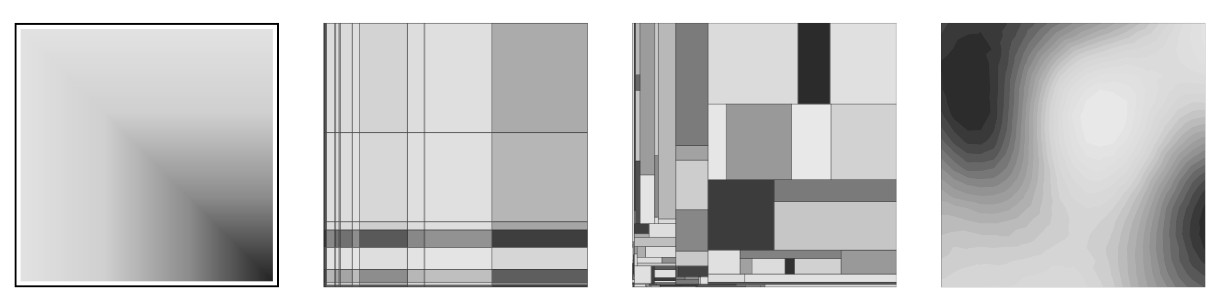
\includegraphics[width = 1\textwidth]{graphons.jpg}
    \caption{Graphons representing different types of random graph models. Left to right: Undirected  graph  with  linear  edge  density ~\parencite{graphlim}, nonparametric block model for separately exchangeable data ~\parencite{infrelmodel}, Mondrian process model for separately exchangeable  data ~\parencite{mondrian}, graphon  with  Gaussian  process  distribution  for  undirected  graph ~\parencite{graphongp}. Figure taken from ~\parencite{exchangeableorbanz}.}
\end{figure}

These exchangeability theorems have a similar format: There is some random exchangeable structure $X$, whether it is a sequence or a graph. Then its respective representation theorem introduces some space $\bs{T}$ and a family of random variable $X_\theta^0$, parametrised by $\theta \in \bs{T}$. $X$ is then exchangeable if and only if

\begin{equation}
    X \overset{d}{=} X_\Theta\quad \text{for some}\, \Theta \in \bs{RV}(\bs{T})
\end{equation}

In practice, the data consists of only a single, large graph. This observed graph with $N$ vertices, $\mc{G}_N$, can be seen as a small subset of an infinite graph $\mc{G}$, just like $N$ observation in a sequential data set can be interpreted as the first $N$ elements of an infinite sequence. Assuming exchangeability, we know there is a random graphon $W$ such that $\mc{G} \overset{d}{=} \mc{G}_W$, explaining our vertices as the first $N$ vertices sampled using \ref{graphon_sample}.

\section{Quadratic Forms In Random Variables} \label{sec:quad}
We are interested in determining the probability density function of the squared distance between two random variables, $X_1$ and $X_2$, governed by the same Gaussian distribution. The squared distance is a random variable, $Y = (X_1 - X_2)^T(X_1 - X_2)$. Since the difference between two Gaussian random variables is itself a Gaussian, we are looking for the probability density function of $U = X^TX$, where $X \sim \mc{N}(\bs{\mu}, \Sigma)$. \\

Theorem 4.2b.1 in~\parencite{mathai} states that the density we are looking for is
\begin{equation}
    \label{pdfquad}
    f(u) = \sumlim{k}{0}{\infty}(-1)^kc_k\frac{u^{\frac{n}{2} + k - 1}}{\Gamma(\frac{n}{2} + k)},\quad 0 < u < \infty
\end{equation}
where
\begin{align}
    c_0 &= \exp\left(-\half\sumlim{j}{1}{n}b_j^2\right)\prodlim{j}{1}{n}(2\lambda_j)^{-\half} \\
    c_k &= \frac{1}{k}\sumlim{r}{0}{k - 1}d_{k-1}c_r,\quad k \leq 1 \label{ck}\\
    d_k &= \half\sumlim{j}{1}{n}(1 - kb_j^2)(2\lambda_j)^{-k},\quad k \leq 1 \label{dk}\\
\end{align}
with $\lambda_j$ being the $j^\text{th}$ eigenvalue of $\Sigma$ and $\bs{b} = P\Sigma^{-\half}\bs{\mu}$, where $P$ is the matrix with its columns equal to the eigenvectors corresponding to the eigenvalues $\{\lambda\}$, so
\begin{equation}
    P^T\Sigma P = \text{diag}(\lambda_1,\,\dots,\,\lambda_n)
\end{equation}

We would ideally like to have the probability density function in \ref{pdfquad} reduced from a series. This is possible only if all the eigenvalues have to the same value and $\bs{b} = \bs{0}$, as the recursive interaction in the definition of the $c_k$ terms leads to complicated expressions that do not reduce to a simple formula. \\

More on this topic can be found in~\parencite{mathai}, chapters 3 and 4.

\chapter{RGG Inference}\label{ch:rgginf}
We look to create a simple setting in which we explore the possibility of using a soft random geometric graph as the latent model. Let us denote the observed data by $\mc{G} = \{X_{ij}\}_{i, j \in [N]}$, where $X_{ij} \in \{0,1\}$ represents the existence of an edge between nodes $i$ and $j$, assuming nothing that would induce any structure in the given graph. Let $X = \{X_i\}_{i \leq N}$ denote the set of latent embeddings of the vertices, $X_i \in \mb{R}^n,\,\forall i \in [N]$. We then model the random variable representing an edge, $X_{ij}$, as a Bernoulli random variable, with mean $e^{-U_{ij}^2}$, where $U_{ij} = \text{dist}(X_i, X_j)$. This stochastic edge makes the model a soft random geometric graph, as referenced in section \ref{sec:rgg}. \\

For some prior on the embeddings $\mb{P}(X)$, we aim to determine the posterior, after observing the data, $\mb{P}(X \mid \mc{G})$. This implies that we need to determine the probability density function of $U_{ij}^2 \mid X_i, X_j \sim \mc{D}$, where $\mc{D}$ represents some prior distribution on the embeddings. We look to approximate the posterior by some variational distribution $q(X) \approx \mb{P}(X \mid \mc{G})$ that we pick ourselves, to circumvent calculating the likelihood $\mb{P}(X)$ and be certain that we choose one which is more accessible to work with. \\ 

\section{Spherical RGG}
When modelling the embeddings as sitting on a hypersphere, we have two possible approaches to measuring the geodesic, the shortest path between two points:
\begin{enumerate}
    \item In a spherical geometry, where the edges are curves on the sphere
    \item In a Euclidean setting, so the edges go through the sphere
\end{enumerate}

In both frameworks, we need to place a prior over the embedding points. Let us assume we are working with a unit-radius hypersphere, though nothing much changes when working with an arbitrary radius. The simplest distribution would be the uniform one, but that is not interesting enough, as it offers no flexibility, so we opt for the von Mises - Fisher distribution, which is akin to the normal distribution, except the points all have a fixed norm, thus they are located on the same hypersphere. Its probability density function is

\begin{equation}
    f_n(\bs{x}; \bs{\mu}, \kappa) = C_n(\kappa) e^{\kappa \bs{\mu}^T \bs{x}}
\end{equation}
where $\kappa > 0$ is the concentration parameter of the distribution around the mean direction $\bs{\mu}$, $\lVert \bs{\mu} \rVert = 1$. The greater $\kappa$ is, the more concentrated the points are, with $\kappa = 0$ determining a uniform distribution. The normalisation constant $C_n(\kappa)$ is
\begin{equation}
    C_n(\kappa) = \frac{\kappa^{\frac{n}{2} - 1}}{(2\pi)^{\frac{n}{2}}I_{\frac{n}{2} - 1}(\kappa)}
\end{equation}
where $I_u$ represents the modified Bessel function of the first kind at order $u$. \\

\begin{figure}[!ht]
    \centering
    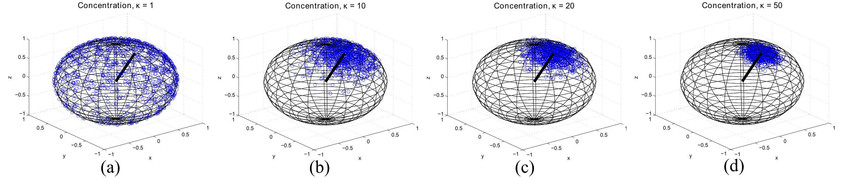
\includegraphics[width = 1\textwidth]{vonMises.jpg}
    \caption{von Mises - Fisher pdf for different concentration parameters, in $\mb{S}_2$. Figure 3 in~\parencite{vonMisesFig}}
\end{figure}

Since only the relative position of the points matters, we can pick any mean direction $\bs{\mu}$, so we can simplify our work by choosing $\bs{\mu} = (1,\,0,\,\dots,\,0)$, leaving only $\kappa$ to vary. We need to find the probability distribution function for the distance between two points governed by a von Mises - Fisher distribution. In the first framework, the distance between two points $\bs{x}_1$ and $\bs{x}_2$ is given by
\begin{equation}
    d = \cos^{-1}(\bs{x}_1^T\bs{x}_2)
\end{equation}
This distance function leads to an intractable integral when calculating the probability density function of the squared distance between two von Mises - Fisher random variables. \\

If we are to work with Euclidean distances, but the embeddings still lying on the hypersphere, the calculations are relatively more approachable, especially since we assume the mean direction to be a convenient one, namely $\bs{\mu} = (1,\,0,\,\dots,\,0)$. Nevertheless, we again run into an integral we cannot solve analytically, rendering this avenue ineffective as well. \\

\section{Hyperbolic RGG}

Hyperbolic geometry is a non-Euclidean geometry referring to spaces of constant negative curvature. Its most famous representative instance is the Minkowski spacetime in special relativity. Hyperbolic spaces started receiving attention in the context of hierarchical data representation due to the fact that they are naturally endowed to model exponential growth. A tree with branching factor $f$ has $(f + 1)f^{l - 1}$ nodes at level $l$ and $\frac{(f+1)f^l-2}{f-1}$ nodes on a level less or equal to $l$, thus the number of children grows exponentially with the distance to the root. This kind of behaviour can be reproduced in hyperbolic geometry using only two dimensions, by placing the nodes at level $l$ on a sphere with radius $R \propto l$, in hyperbolic space. This can be done because hyperbolic spaces grow exponentially with distance, as opposed to their Euclidean counterparts, for which the circle area grows quadratically with the radius. \\

The work of Krioukov et al. in~\parencite{krioukov} paved the way for the usage of the hyperbolic space as a space to represent trees, proving that one can interpret them as a discrete version of a hyperbolic space. This served as a basis for ~\parencite{poincare}, a paper that details a method of embedding the \texttt{WORDNET}~\parencite{wordnet} noun hierarchy, which is structured as a tree, hence the obvious latent hierarchical setting. The difficulty of representing spaces of constant negative curvature as subsets of Euclidean spaces leads to multiple equivalent models of hyperbolic spaces, each capturing different aspects of the geometry, but no single model encapsulating all of them. For example, the hyperboloid model is usually used in special relativity, and projecting it in two different ways to disks orthogonal to its main axis yields the Poincar\'{e} and Klein unit disks models. Krioukov uses the native representation in his analysis, such that all distance variables have their true hyperbolic values. While the first embeddings of Nickel and Kiela ~\parencite{poincare} lie in the Poincar\'{e} hyperbolic space, other papers use equivalent models ~\parencite{skipgram, lorentz}. The field of NLP relies heavily on embeddings, so it was natural to extend some of the methods of embeddings words, namely \texttt{GLOVE}~\parencite{glove} and \texttt{SKIPGRAM}~\parencite{word2vec}, to the hyperbolic spaces, as seen in~\parencite{skipgram, poincareglove}. Adaptations to working with matrices in the Poincar\'{e} disk model have made it possible to use hyperbolic embeddings in deep learning ~\parencite{hnn, ahnn}, although the field is still in its infancy. \\

The aforementioned work treats the embeddings algorithmically, without placing a prior over them, and, trying to do that, we can see where the difficulty lies. Working in the two dimensional hyperbolic space of curvature $-\xi^2$, $\mb{H}_\xi$, like Krioukov ~\parencite{krioukov}, and representing points using their polar coordinates, we have that the distance $x$ between two points $(r, \theta)$ and $(r', \theta')$ is equal to

\begin{equation}
    d = \frac{1}{\xi}\cosh^{-1}(\cosh(\xi r)\cosh(\xi r') - \sinh(\xi r)\sinh(\xi r')\cos(\Delta\theta))
\end{equation}
where $\Delta\theta = \pi - |\pi - |\theta - \theta'||$. This complicated formula makes it impossible to obtain a closed form for the probability density function corresponding to the distance between two hyperbolic points, for any sensible, non-trivial prior on the points. The same is true for the Poincar\'{e} ball of curvature -1, where the distance between two points $x$ and $y$ is

\begin{equation}
    d = \cosh^{-1}\left(1 + \frac{2\lVert x - y \rVert^2}{(1 - \lVert x \rVert^2)(1 - \lVert y \rVert^2)}\right)
\end{equation}

This space, while endowed with the ability to encode tree-like structures, as opposed to the Euclidean space, which cannot preserve the metric of arbitrary tree structures, even in infinite dimensions ~\parencite{representation}, comes with metrics that do not lead to a clean probability density function for non-trivial priors on the embeddings, deeming this avenue unfeasible.

\section{Euclidean RGG}
We can start by assuming a simple multivariate Gaussian prior for the embeddings. Since their absolute position is irrelevant, we can simply choose the mean to be $\bs{\mu}_0 = \bs{0}$. As for the covariance matrix, let it be some generic $\Sigma_0$ for the time being. We aim to approximate the posterior $\mb{P}(\bs{X} \mid \mc{G}),\, \bs{X} = \{X_i\}_{i \in [N]}$ by a multivariate Gaussian, again with mean $\bs{\mu} = \bs{0}$ and some covariance matrix $\Sigma$, hence the approximating distribution $q$,
\begin{align*}
    q(\bs{X}) &\approx \mb{P}(\bs{X} \mid \mc{G}) \\
    \bs{X} &\overset{q}{\sim} \mc{N}(\bs{0}, \Sigma)
\end{align*}

Working in a variational inference setting, we can rewrite equation \ref{free_energy} for the free energy as
\begin{align*}
    \mc{F}(\sigma) = \left<\log\mb{P}(\mc{G} \mid \bs{X})\right>_{q(\bs{X})} - KL[q(\bs{X}) \mid\mid \mb{P}(\bs{X})]
\end{align*}

Le us focus on the first term for now, denoting the value of the square distance between two Gaussian embeddings by $u_{ij} = \text{dist}(X_i, X_j)^2$, and capitalising it to represent the random variable associated with it. We need to integrate over the distances between the pairs of embeddings, instead of the embeddings themselves, thus we rewrite
\begin{align*}
    \left<\log\mb{P}(\mc{G} \mid \bs{X})\right>_{q(\bs{X})} &= \int\limits_{(\mb{R}^n)^N} q(\bs{X})\log\mb{P}(\mc{G} \mid \bs{X}) d\bs{X} \\
    &= \int\limits_{(\mb{R}^n)^N} q(\bs{X}) \prodl{i<j} e^{-u_{ij}X_{ij}}(1 - e^{-u_{ij}})^{1 - X_{ij}} \\
    &= \suml{i<j}\int\limits_{(\mb{R}_{>0})^\frac{N(N-1)}{2}} q(\bs{U}) (-u_{ij}X_{ij} + (1 - X_{ij})\log(1 - e^{-u_{ij}})) d\bs{U} \\
    &= \suml{i<j}\int\limits_{\mb{R}_{>0}} q(u_{ij}) (-u_{ij}X_{ij} + (1 - X_{ij})\log(1 - e^{-u_{ij}})) du_{ij} \\
    &= \suml{i<j}\int\limits_{\mb{R}_{>0}} q(u_{ij}) \left(-u_{ij}X_{ij} + (1 - X_{ij})\log\frac{e^{u_{ij}} - 1}{e^{u_{ij}}}\right) du_{ij} \\
    &= \suml{i<j}\int\limits_{\mb{R}_{>0}} q(u_{ij}) (-u_{ij}X_{ij} - (1 - X_{ij})u_{ij} + (1 - X_{ij})\log(e^{u_{ij}} - 1)) du_{ij} \\
    &= \suml{i<j}\int\limits_{\mb{R}_{>0}} q(u_{ij}) (-u_{ij} + (1 - X_{ij})\log(e^{u_{ij}} - 1)) du_{ij} \\
    &= -\comb{N}{2}<u>_{q(u)} + \suml{i<j}(1 - X_{ij})\int\limits_{\mb{R}_{>0}} q(u_{ij}) \log(e^{u_{ij}} - 1) du_{ij} \\
    &= -\comb{N}{2}<u>_{q(u)} + \left(\comb{N}{2} - \ub{E}_{\text{\#edges}}\right)\int\limits_{\mb{R}_{>0}} q(u) \log(e^{u} - 1) du
\end{align*}

We now have to calculate the probability density function of the squared distance between two random multivariate normal variables. As presented in section \ref{sec:quad}, in order to obtain a closed formula, we need to make some assumptions. We have already set $\bs{\mu} = \bs{0}$, so now we have to choose $\Sigma$ such that the eigenvalues all have the same value, therefore we set $\Sigma = \sigma^2\mc{I}$, leading to
\begin{equation*}
    q(u) = \frac{u^{m-1}(2\sigma^2)^{-m}}{(m-1)!}\exp(-(2\sigma^2)^{-1}u)
\end{equation*}
During the calculation we make an extra assumption, such that $n$ is even, $n = 2m,\,m \in \mb{N}$. The full work can be found in appendix~\ref{appendix}. We then have
\begin{align*}
    \left<\log\mb{P}(\mc{G} \mid \bs{X})\right>_{q(\bs{X})} &= -\comb{N}{2}2m\sigma^2 + \left(\comb{N}{2} - E\right)\frac{(2\sigma^2)^{-m}}{(m-1)!}\int\limits_{\mb{R}_{>0}} u^{m-1}\exp(-(2\sigma^2)^{-1}u) \log(e^{u} - 1) du
\end{align*}

The integral does not have a closed form, so we are forced to approximate it using Riemann sums. Since the function under the integral converges to 0 as $u$ increases, we need to identify a large enough value of $u$ such that the function is close enough to $0$. \\

The KL divergence between two multivariate Gaussians of dimension $n$, $\mc{N}(\mu_1, \Sigma_1)$ and $\mc{N}(\mu_2, \Sigma_2)$ equals
\begin{equation}
    \half\left[\log\frac{|\Sigma_2|}{|\Sigma_1|} - n + \text{tr}[\Sigma_2^{-1}\Sigma_1] + (\mu_2 - \mu_1)^T\Sigma_2^{-1}(\mu_2 - \mu_1)\right]
\end{equation}

The hyperparameters for the approximate distribution $q$ and the prior $\mb{P}$ are usually optimised together. However, because the hyperparameters of the prior only appear in the KL divergence term, their optimal value equals the value of the hyperparameters of $q$. We therefore employ a constant prior and set $\Sigma_0 = \mc{I}$, the identity matrix. The free energy then becomes

\begin{align*}
    \mc{F}(\sigma) &= -\comb{N}{2}2m\sigma^2 + \left(\comb{N}{2} - E\right)\frac{(2\sigma^2)^{-m}}{(m-1)!}\int\limits_{\mb{R}_{>0}} u^{m-1}\exp(-(2\sigma^2)^{-1}u) \log(e^{u} - 1) du \\
    &- Nm(-\log(\sigma^2) - 1 + \sigma^2)
\end{align*}
leaving us to optimise $\sigma$ only. We can do this by gradient descent, but experiments showed that a fixed step size does not work well for all experiments, unless it very small. However, noticing that the free energy is concave with respect to $\sigma$, we can employ binary search to find the value that maximises it. \\

\subsection{Relation To Graphons}

A special case of the Borel isomorphism theorem allows us to map a Uniform[0, 1] random variable to a multivariate Gaussian, which allows us to work with the latter when generating graphs. Let $\phi : [0,\,1] \rightarrow \mb{R}^n$ be that mapping. If we work with the squared distance between embeddings to randomly determine the existence of an edge, the graphon we are working with is
\begin{equation}
    w(x, y) = e^{-(\phi (x) - \phi (y))^T(\phi (x) - \phi (y))}
\end{equation}

It is important to state that if the embedding space is fixed, as it is the case in our model, the data can be considered exchangeable, but if the space grows with the number of vertices, then the exchangeability property is broken. Recall that the exchangeability amounts to the probability of seeing the data does not change when we swap two vertices, assuming that our data consists of a finite number of elements from an infinite structure. But if the embedding space changes with the number of data points seen, then seeing the value of the last embedding as the first might be impossible or arise with a different probability, hence the lack of exchangeability. \\

\subsection{Synthetic Experiments}
Assessing model fitness on graph data is not straightforward. For other types of data, cross-validation is usually employed, but using it in a network setting implies subsampling the observed graph, which induces strong assumptions on how the data was generated. \\

Therefore, we use a protocol devised by Hunter et al. in~\parencite{hunter}, where models are compared to the data by fixing a set of graph statistics. A fitted model is evaluated by using it to simulate a network, then comparing its statistics with those of the original data. The following statistics presented in~\parencite{hunter} capture a range of structures:
\begin{itemize}
    \item normalised degree statistics $d_k$, the number of vertices of degree $k$, divided by the total number of vertices;
    \item normalised edgewise shared partner statistics $\chi_k$, the number of unordered connected pairs $\{i,\,j\}$ with exactly k common neighbours, divided by the total number of edges;
    \item normalized pairwise geodesic statistics $\gamma_k$ , the number of unordered pairs $\{i,\, j\}$ with distance $k$ in the graph, divided by the number of dyads.
\end{itemize}

We also include the number of edges, since the variance $\sigma^2$ on each dimension directly determines how close points are, thus modulating the presence of edges. Working in a Bayesian setting, implementing the protocol corresponds to performing posterior predictive checks ~\parencite{box, gelman} in the following manner
\begin{itemize}
    \item Sample the latent embeddings from the approximate posterior, $q(X) \approx \mb{P}(X \mid \mc{G})$;
    \item Simulate a graph using the embeddings, $\mc{G}^{(s)} \sim \mb{P}(\mc{G} \mid X)$;
    \item Calculate the statistics of interest in the simulated graph.
\end{itemize}

The tables below list the total variation distances between the empirical distribution of each statistic of the observed graph and on the graphs generated from the learnt model. For discrete distributions $P$ and $Q$ with sample space $\Omega$, this distance is calculated as ~\parencite{tvd}:
\begin{equation}
    \delta(P, Q) = \half\sum\limits_{\omega \in \Omega}|P(\omega) - Q(\omega)|
\end{equation}

Each experiment is run with 300 vertices, and the standard errors are computed over 20 runs, smaller values indicating better fits. We employ various distributions to generate data, representing the vertices, and then draw edges stochastically, based on the distance between them, as presented in the beginning of Chapter \ref{ch:rgginf}. The resulting adjacency matrix is then used as data for our model. \\

By \textit{Original Edges} and \textit{Model Edges} we mean the number of edges of the original geometric graph and the simulated graph using the inferred parameter $\sigma$, respectively. \textit{TVD} refers to the total variation distance for the statistics corresponding to the original graph and the ones of the model. \\

We start off by generating graphs using a spherical multivariate normal distribution in two dimensions and trying to recover the variance. An example of how such a graph might look can be seen in figure \ref{fsphericalg}, albeit for 100 nodes. Table \ref{tsphericalg} shows that the parameter is recovered fairly well for smaller values, but, as $\sigma$ increases, the recovered parameter does not increase at the same rate, leading to more than five times the number of edges, compared to the original data. \\

\begin{table}[!ht]
    \centering
    \tiny
    \csvreader[tabular=lllllll,
        head=false,
        late after line=\\,
        late after first line=\\\midrule,
        table foot=\bottomrule,
        ]{test_spherical_gaussian_m1.csv}{}{\csvcoli & \csvcolii & \csvcoliii & \csvcoliv & \csvcolv & \csvcolvi & \csvcolvii}
    \caption{Spherical Gaussian data with covariance matrix $\sigma^2\mc{I}_2$}
    \label{tsphericalg}
\end{table}

\begin{figure}[!ht]
    \centering
    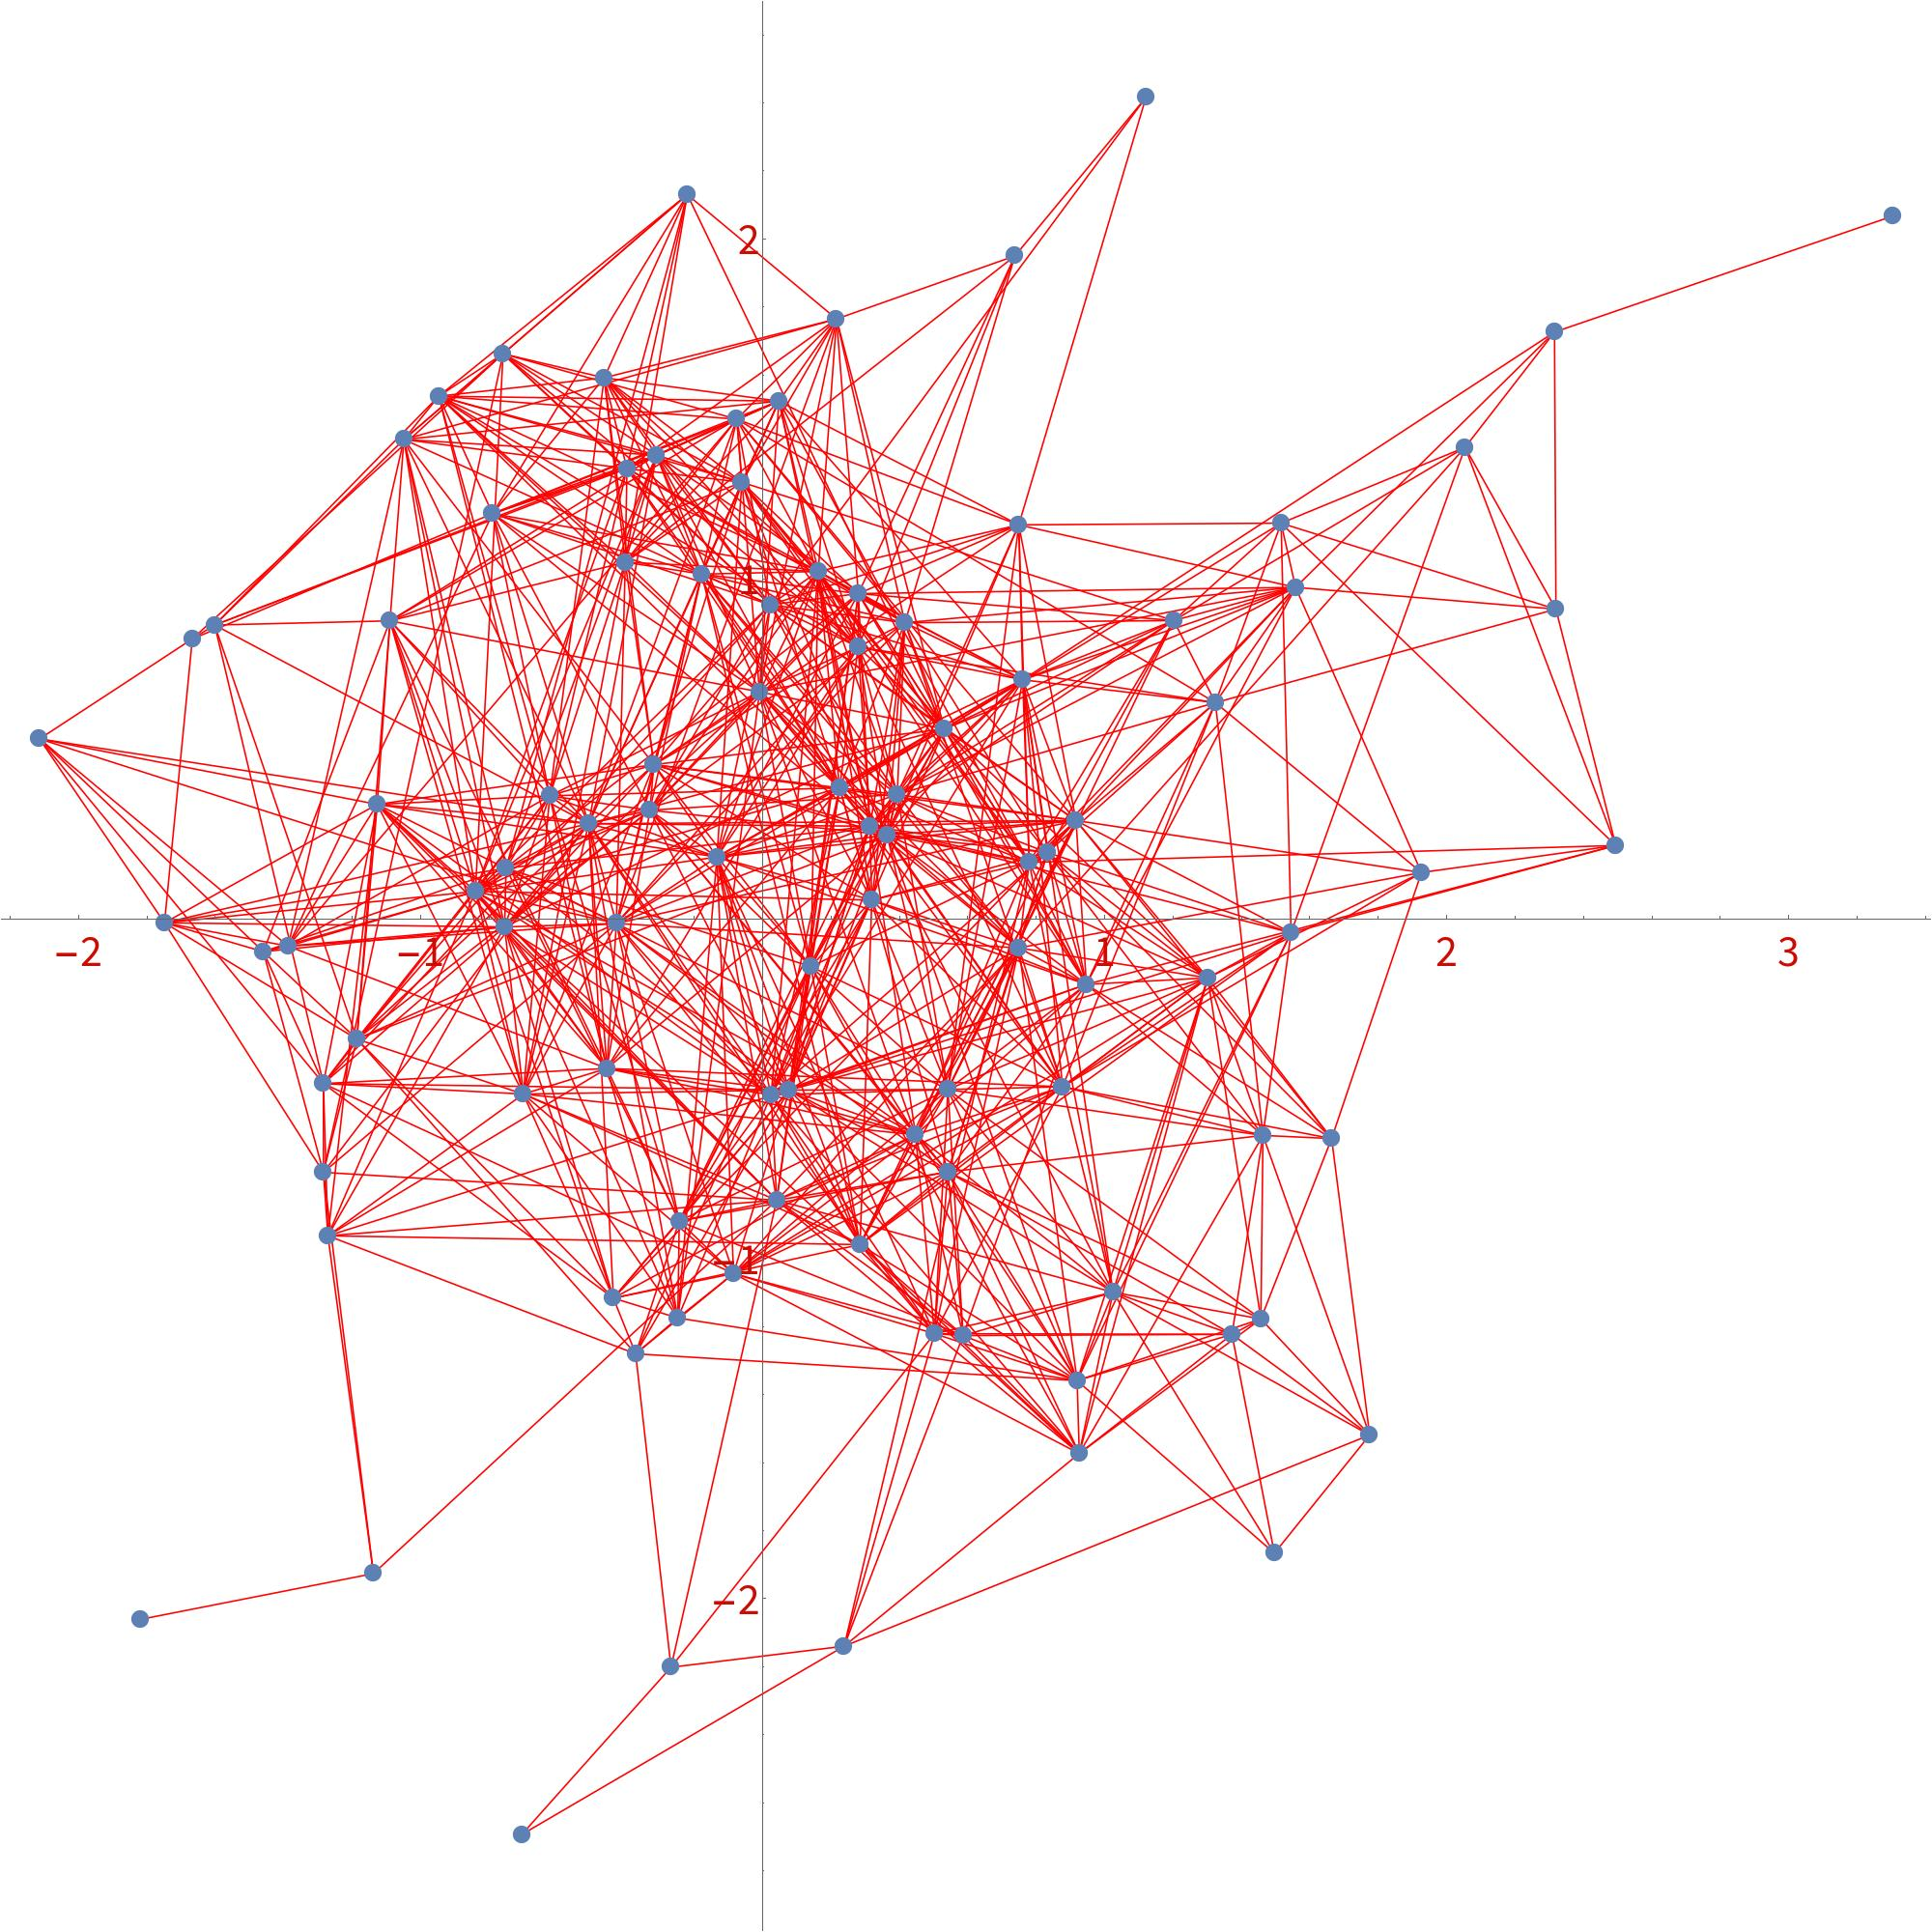
\includegraphics[width = 0.3\textwidth]{gaussian1.jpg}
    \caption{Soft random geometric graph using a multivariate Gaussian distribution with covariance matrix $\mc{I}$ to sample the nodes}
    \label{fsphericalg}
\end{figure}

Table \ref{tsphericalt} contains results for synthetic data generated using a multivariate Student t distribution, which gives rise to sparser graphs than the ones generated using a normal distribution, due to the fatter tail in the probability density function. We can see again that the model severly underestimates the parameter, especially as $\sigma$ grows larger. \\

\begin{table}[!ht]
    \centering
    \tiny
    \csvreader[tabular=lllllll,
        head=false,
        late after line=\\,
        late after first line=\\\midrule,
        table foot=\bottomrule,
        ]{test_spherical_multivariate_t_m1.csv}{}{\csvcoli & \csvcolii & \csvcoliii & \csvcoliv & \csvcolv & \csvcolvi & \csvcolvii}
    \caption{Spherical Multivariate T with covariance matrix $\sigma^2\mc{I}$ and 15 degrees of freedom}
    \label{tsphericalt}
\end{table}

\begin{figure}[!ht]
    \centering
    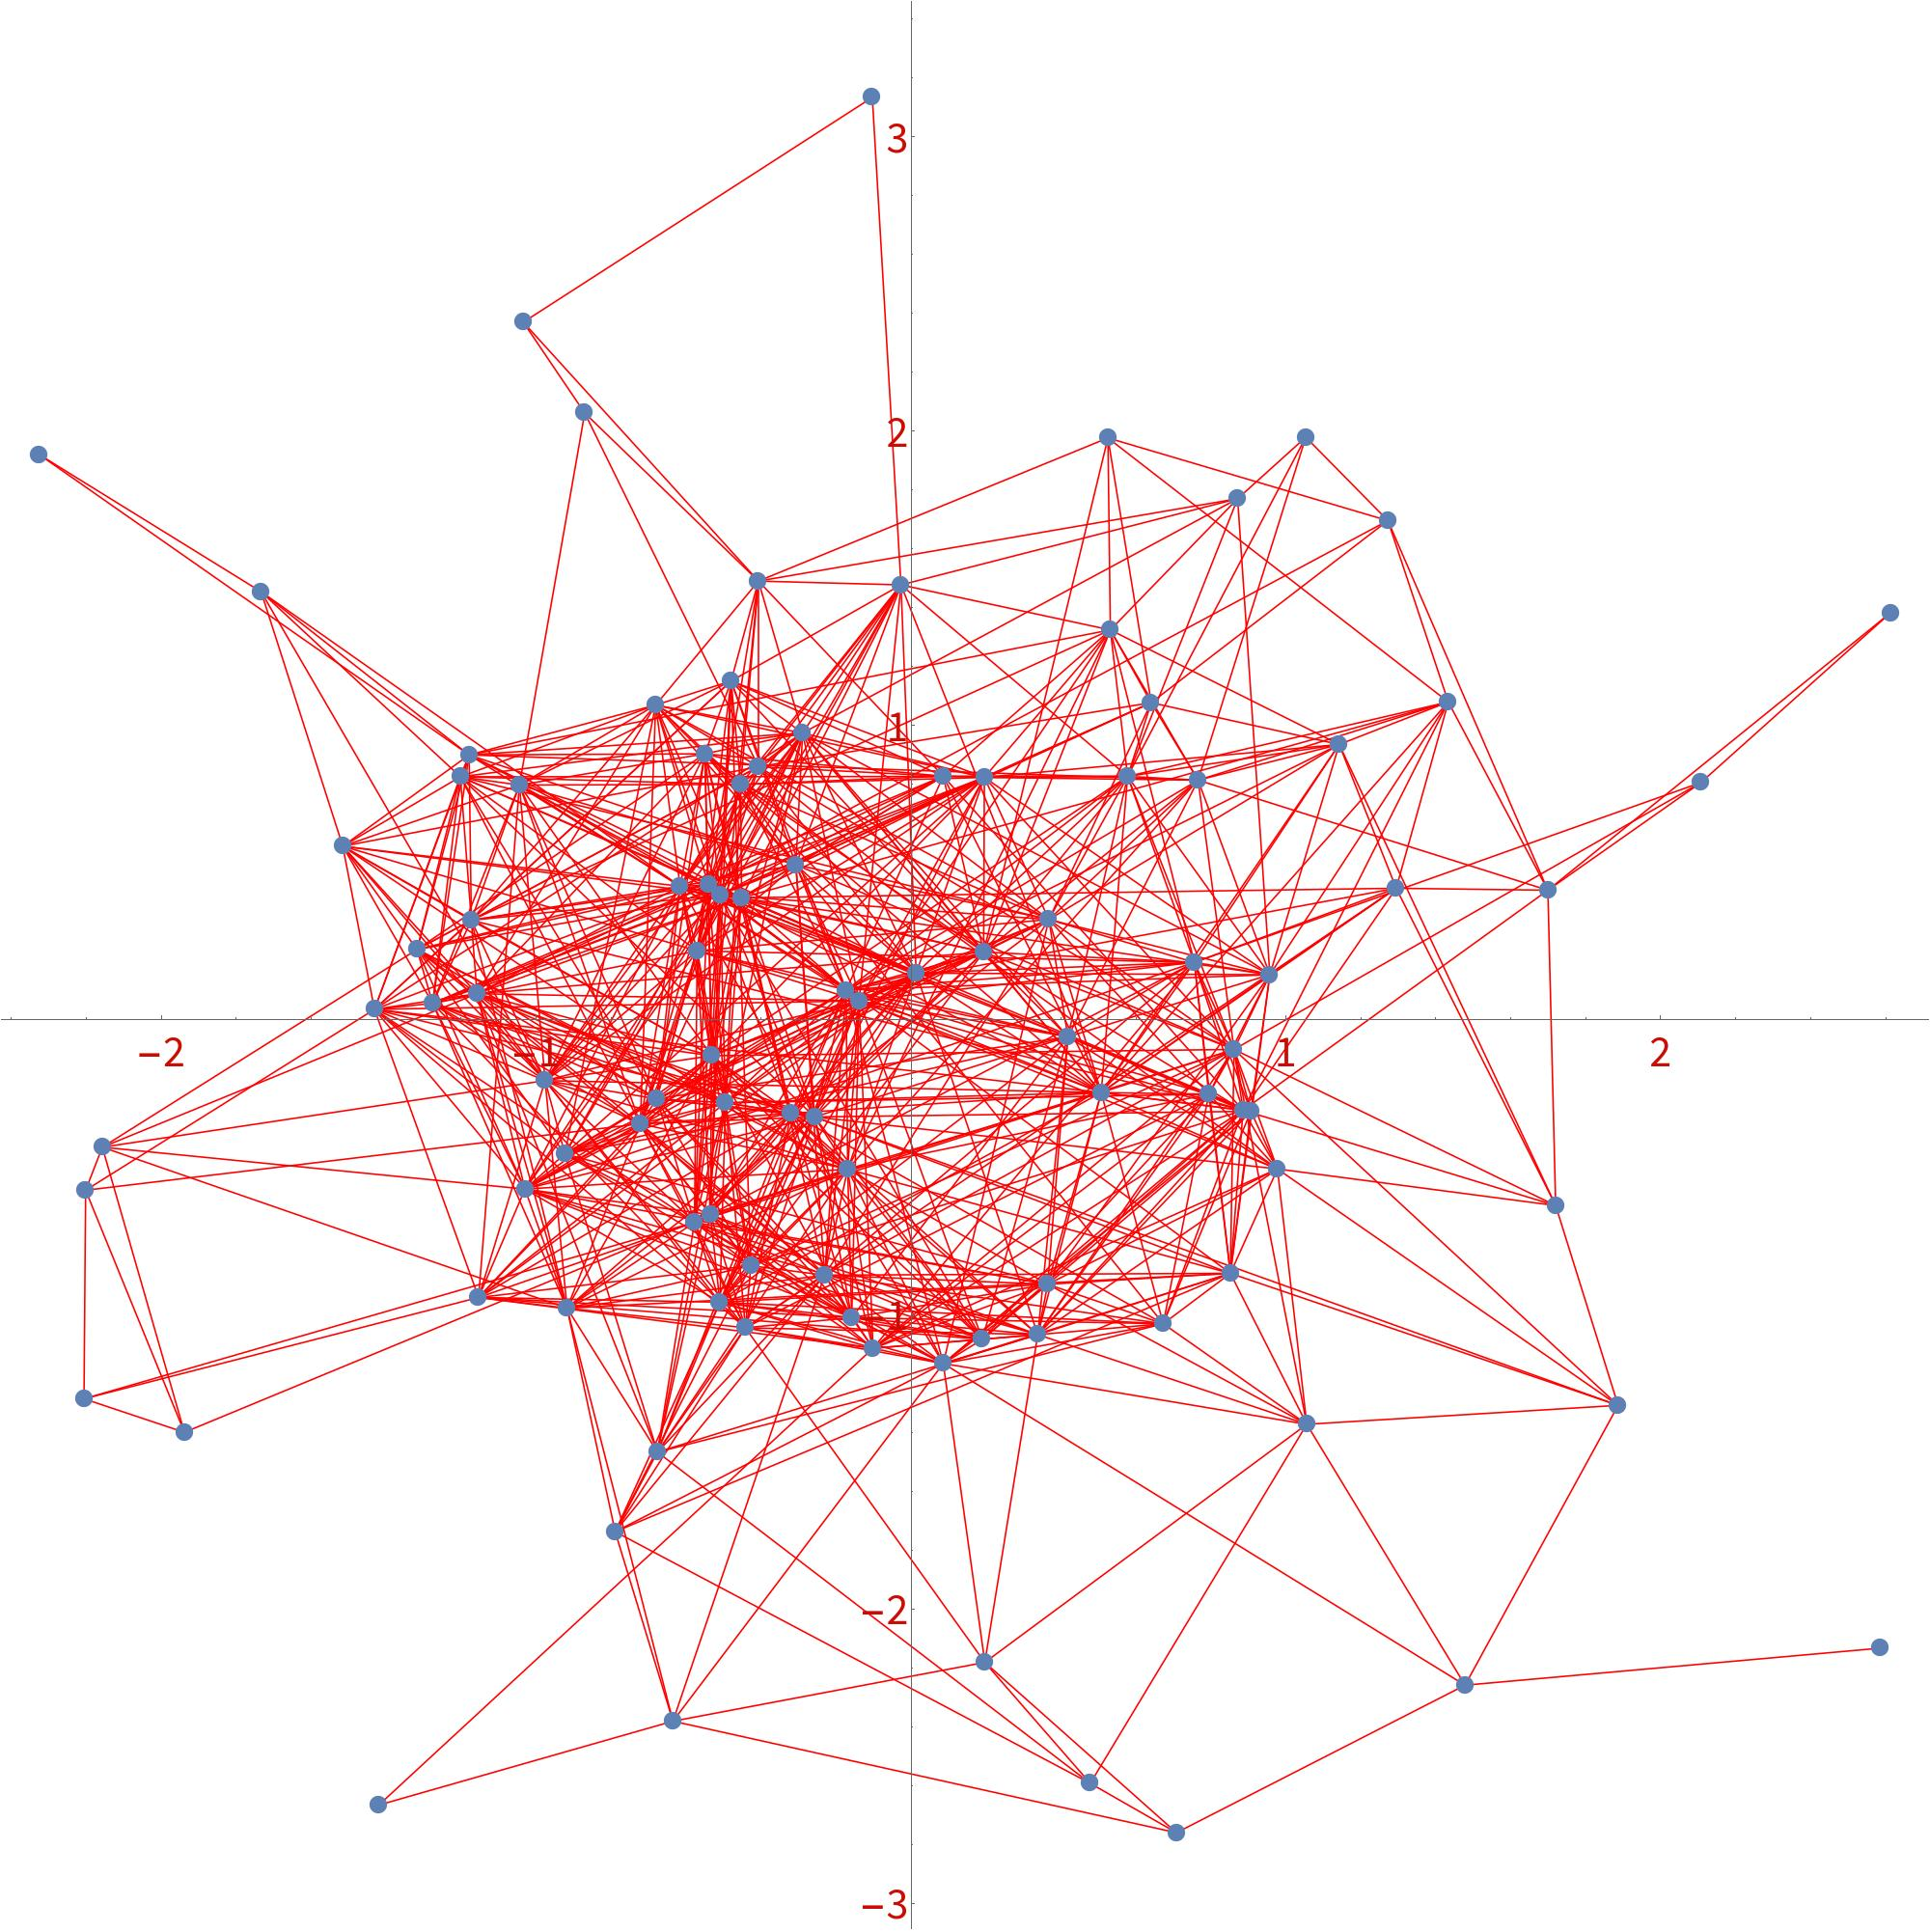
\includegraphics[width = 0.3\textwidth]{multivariatet.jpg}
    \caption[Spherical Multivariate T with 15 degrees of freedom]{Multivariate T with $\Sigma = \mc{I}$ and 15 degrees of freedom.}
\end{figure}

The tables \ref{tmixclose} and \ref{tmixfar} contain results for data generated by a mixture of two normal distributions. The former has the distributions closer together, so the shorter distances between nodes leads to edges between vertices generated by different Gaussians, while the latter places the means further apart, resulting in two components that do not communicate. The total variation distances for the $d_k$ and $\chi_k$ statistics are comparable, but there is a sharp increase for $\gamma_k$, when moving from the mixture with the distributions closer together to the one that has them further apart. This is expected, since $\gamma_k$ is based on the shortest distances between all pairs of nodes and the separate components give rise to a significant number of pairs that do not communicate, and this behaviour cannot be reliably captured by a spherical Gaussian posterior. \\

\begin{figure}[!ht]
\centering
\begin{subfigure}{.5\textwidth}
    \centering
    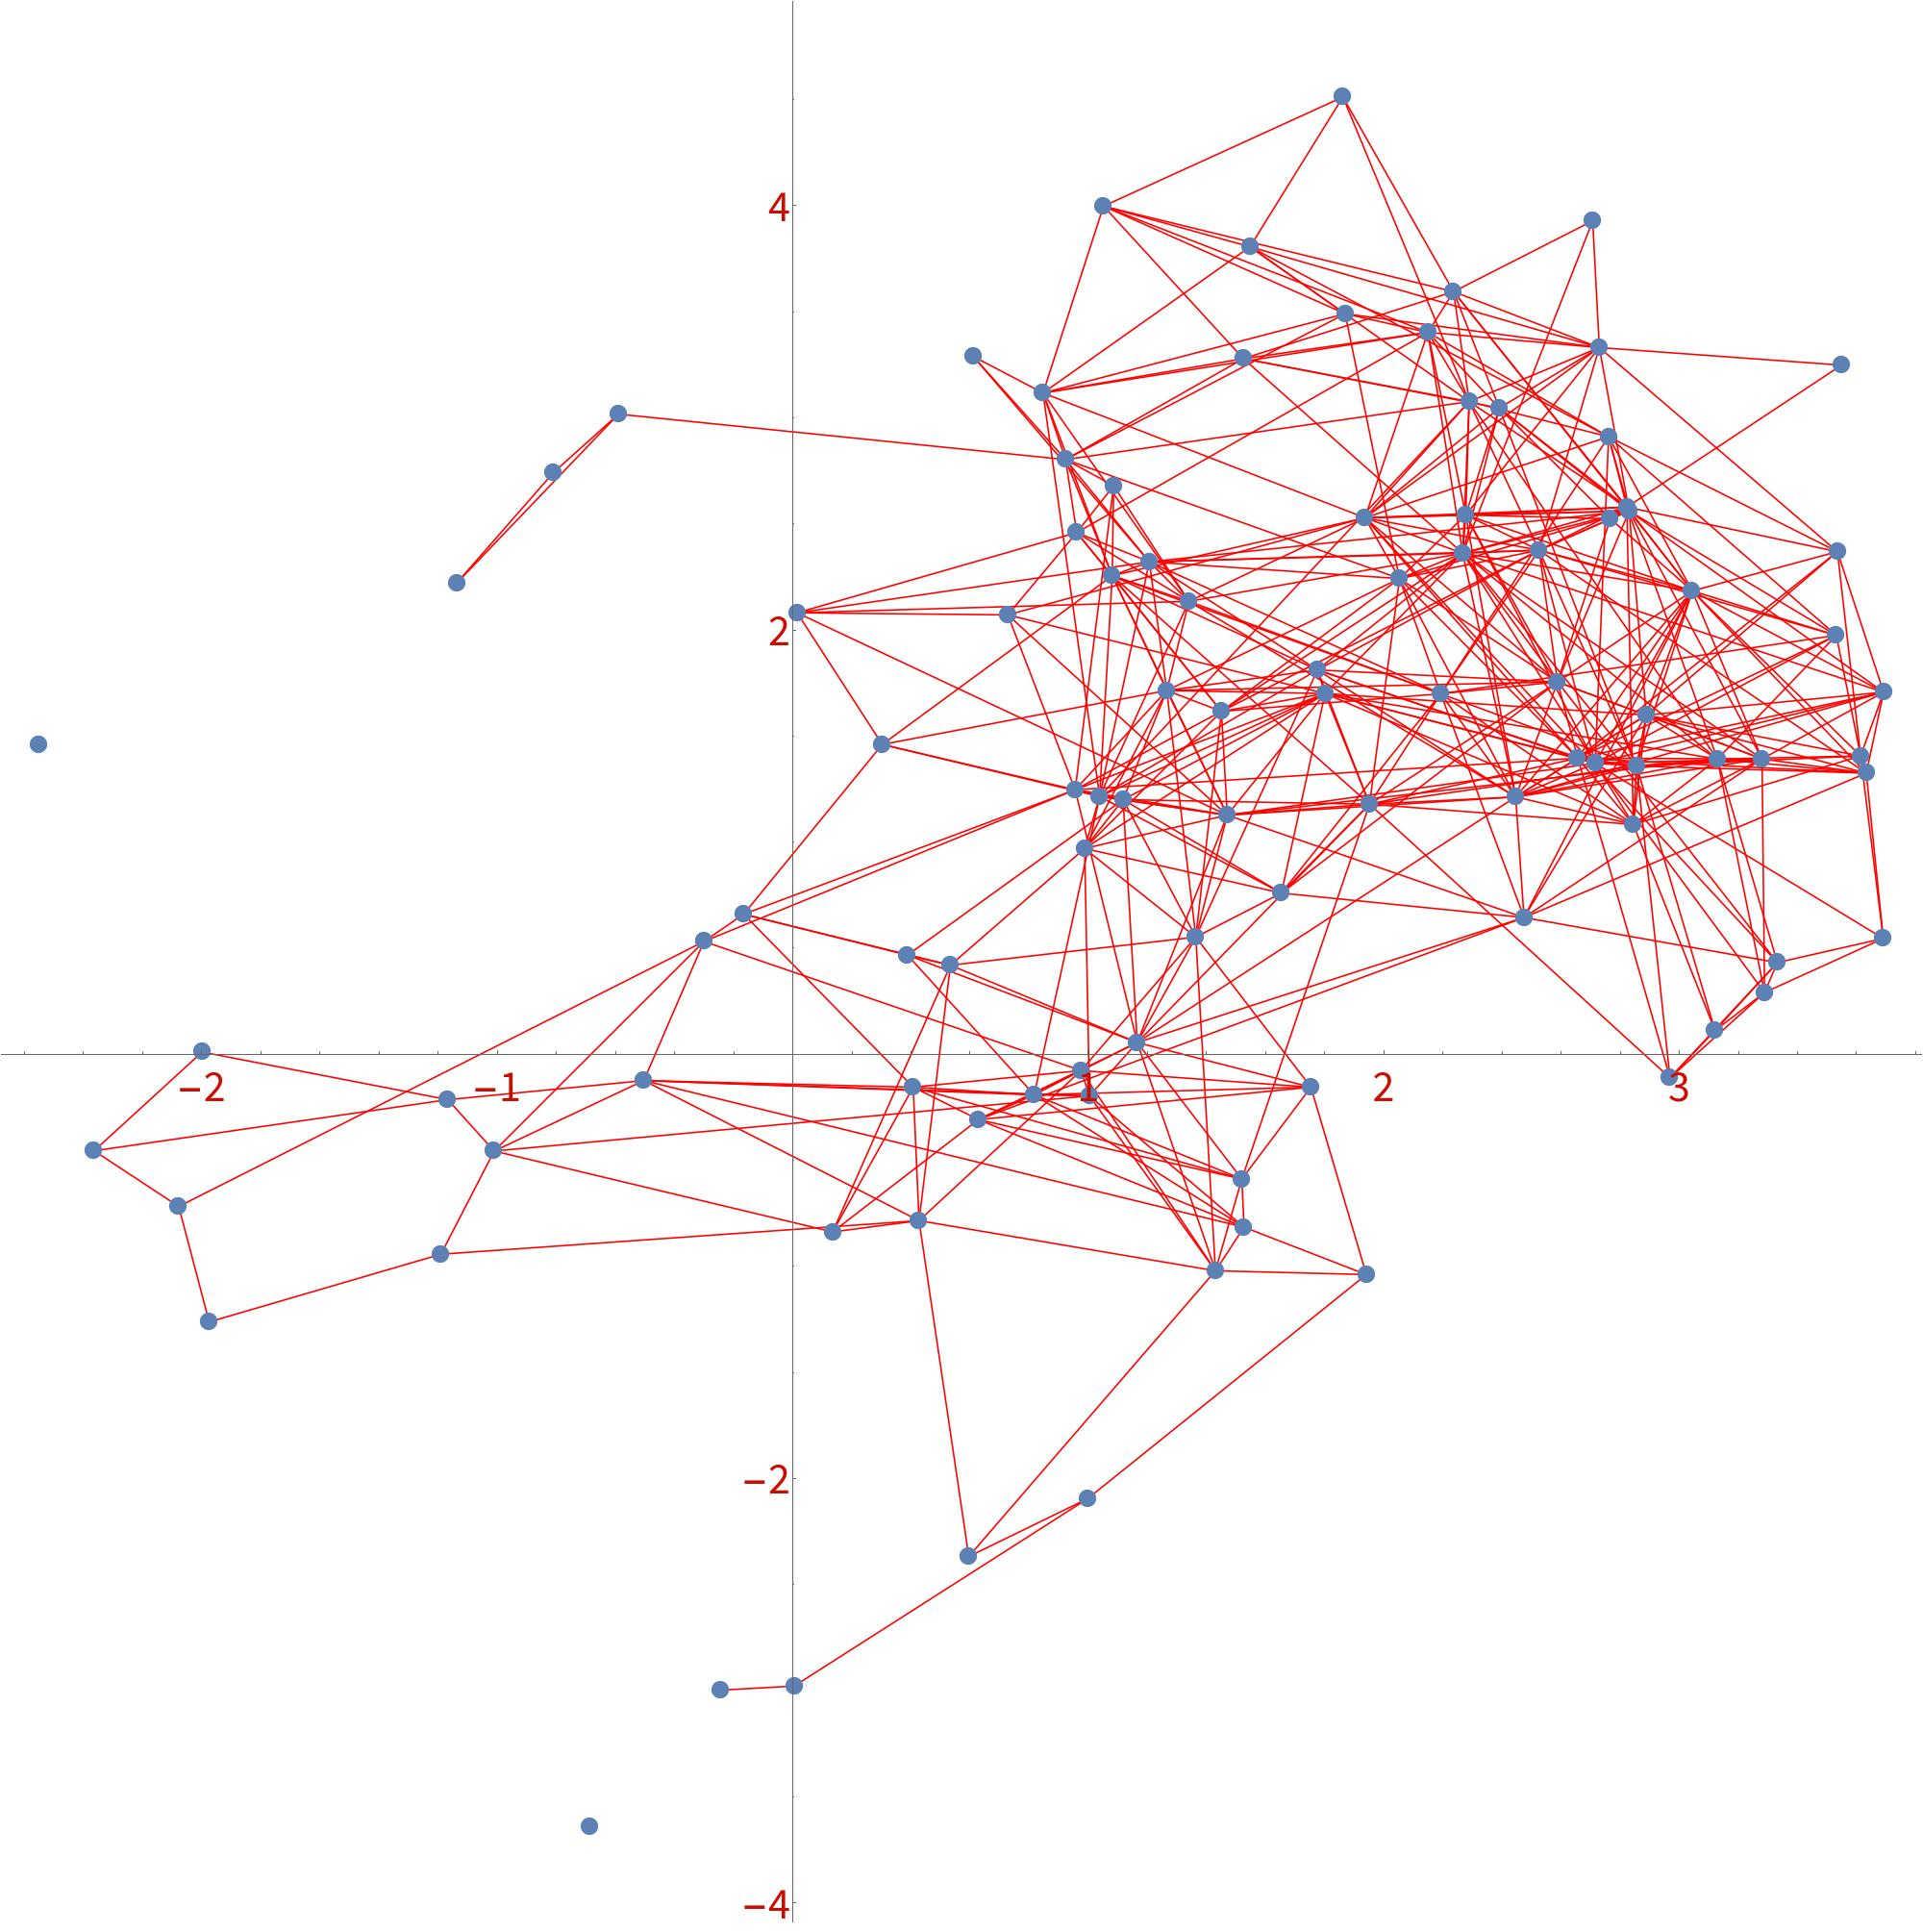
\includegraphics[width = 0.5\textwidth]{gaussian_mixtures.jpg}
    \caption{Mixture of two Gaussians, $\mu_1 = (0, 0),\\ \mu_2 = (2, 2)$, $\Sigma_1 = 1.5\mc{I},\, \Sigma_2 = \mc{I}$, $\mb{\pi} = (0.4, 0.6)$}
    \label{fmixclose}
\end{subfigure}%
\begin{subfigure}{.5\textwidth}
    \centering
    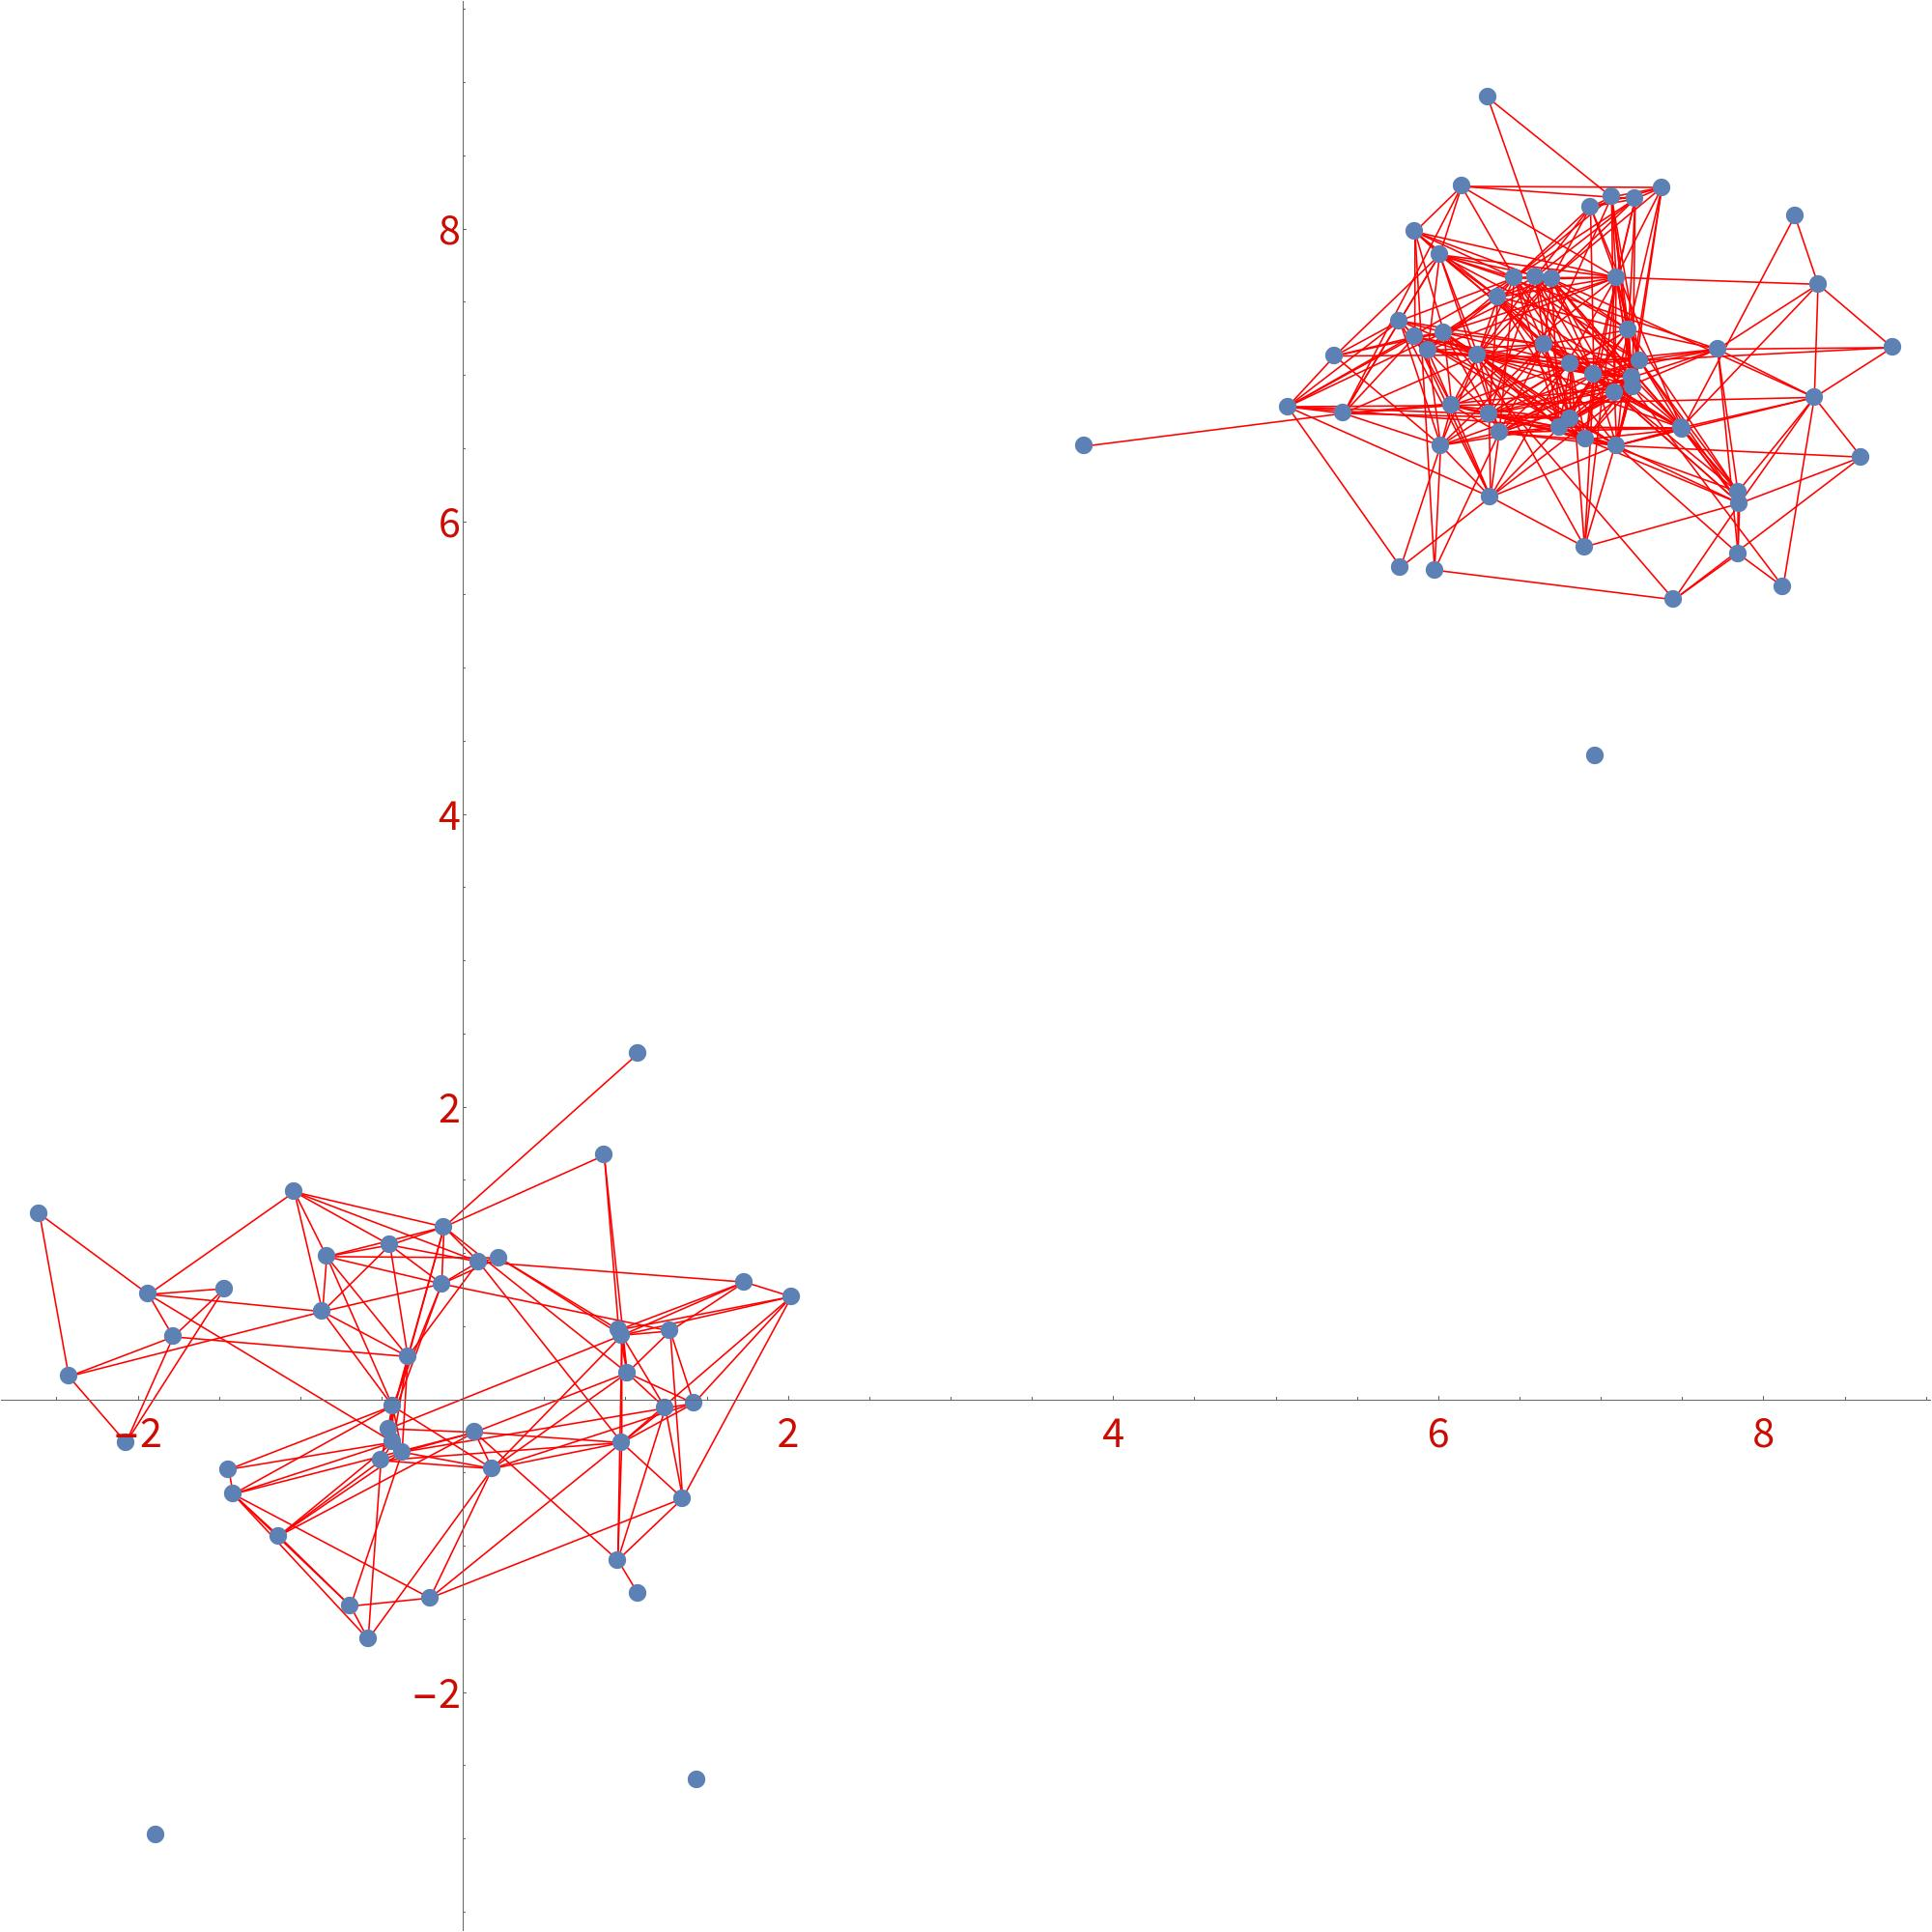
\includegraphics[width = 0.5\textwidth]{gaussian_mixtures_far.jpg}
    \caption{Mixture of two Gaussians, $\mu_1 = (0, 0),\\ \mu_2 = (2, 2)$, $\Sigma_1 = 1.5\mc{I},\, \Sigma_2 = \mc{I}$, $\mb{\pi} = (0.4, 0.6)$}
    \label{fmixfar}
\end{subfigure}
\end{figure}

\begin{table}[!ht]
    \centering
    \tiny
    \csvreader[tabular=llllll,
        head=false,
        late after line=\\,
        late after first line=\\\midrule,
        table foot=\bottomrule,
        ]{test_close.csv}{}{\csvcoli & \csvcolii & \csvcoliii & \csvcoliv & \csvcolv & \csvcolvi}
    \caption{Mixture of two Gaussians, centered at $\mu_1 = (0, 0)$ and $\mu_2 = (2, 2)$, with covariance matrices $1.5\mc{I}$ and $\mc{I}$, and mixing distribution $\pi = (0.4,\,0.6)$.}
    \label{tmixclose}
\end{table}

\begin{table}[!ht]
    \centering
    \tiny
    \csvreader[tabular=llllll,
        head=false,
        late after line=\\,
        late after first line=\\\midrule,
        table foot=\bottomrule,
        ]{test_far.csv}{}{\csvcoli & \csvcolii & \csvcoliii & \csvcoliv & \csvcolv & \csvcolvi}
    \caption{Mixture of two Gaussians, centered at $\mu_1 = (0, 0)$ and $\mu_2 = (7, 7)$, with covariance matrices $1.5\mc{I}$ and $\mc{I}$, and mixing distribution $\pi = (0.4,\,0.6)$.}
    \label{tmixfar}
\end{table}

Tables \ref{tskewedg} and \ref{tskewedt} contain results for data generated by a non-spherical Gaussian and a non-spherical Student t distribution, respectively. When comparing the total variation distance for $\gamma_k$ to those of $d_k$ and $\chi_k$, its value is larger than that of a similar graph, in terms of number of edges, generated by a spherical Gaussian or Student t. This can be attributed to the greater diameter of the structure on its widest dimension, leading to a greater mass on higher geodesic values. \\

\newpage
\begin{table}[!ht]
    \centering
    \tiny
    \csvreader[tabular=llllll,
        head=false,
        late after line=\\,
        late after first line=\\\midrule,
        table foot=\bottomrule,
        ]{test_skewed_g.csv}{}{\csvcoli & \csvcolii & \csvcoliii & \csvcoliv & \csvcolv & \csvcolvi}
    \caption[Gaussian with non-diagonal covariance matrix]{Gaussian with covariance matrix $\begin{pmatrix} 3 & 1.5 \\ 1.5 & 1 \end{pmatrix}$ }
    \label{tskewedg}
\end{table}

\begin{table}[!ht]
    \centering
    \tiny
    \csvreader[tabular=llllll,
        head=false,
        late after line=\\,
        late after first line=\\\midrule,
        table foot=\bottomrule,
        ]{test_skewed_t.csv}{}{\csvcoli & \csvcolii & \csvcoliii & \csvcoliv & \csvcolv & \csvcolvi}
    \caption[Multivariate T with non-diagonal covariance matrix]{Multivariate T with 5 degrees of freedom and covariance matrix $\begin{pmatrix} 3 & 1.5 \\ 1.5 & 1 \end{pmatrix}$ }
    \label{tskewedt}
\end{table}

\begin{figure}[!ht]
\centering
\begin{subfigure}{.5\textwidth}
    \centering
    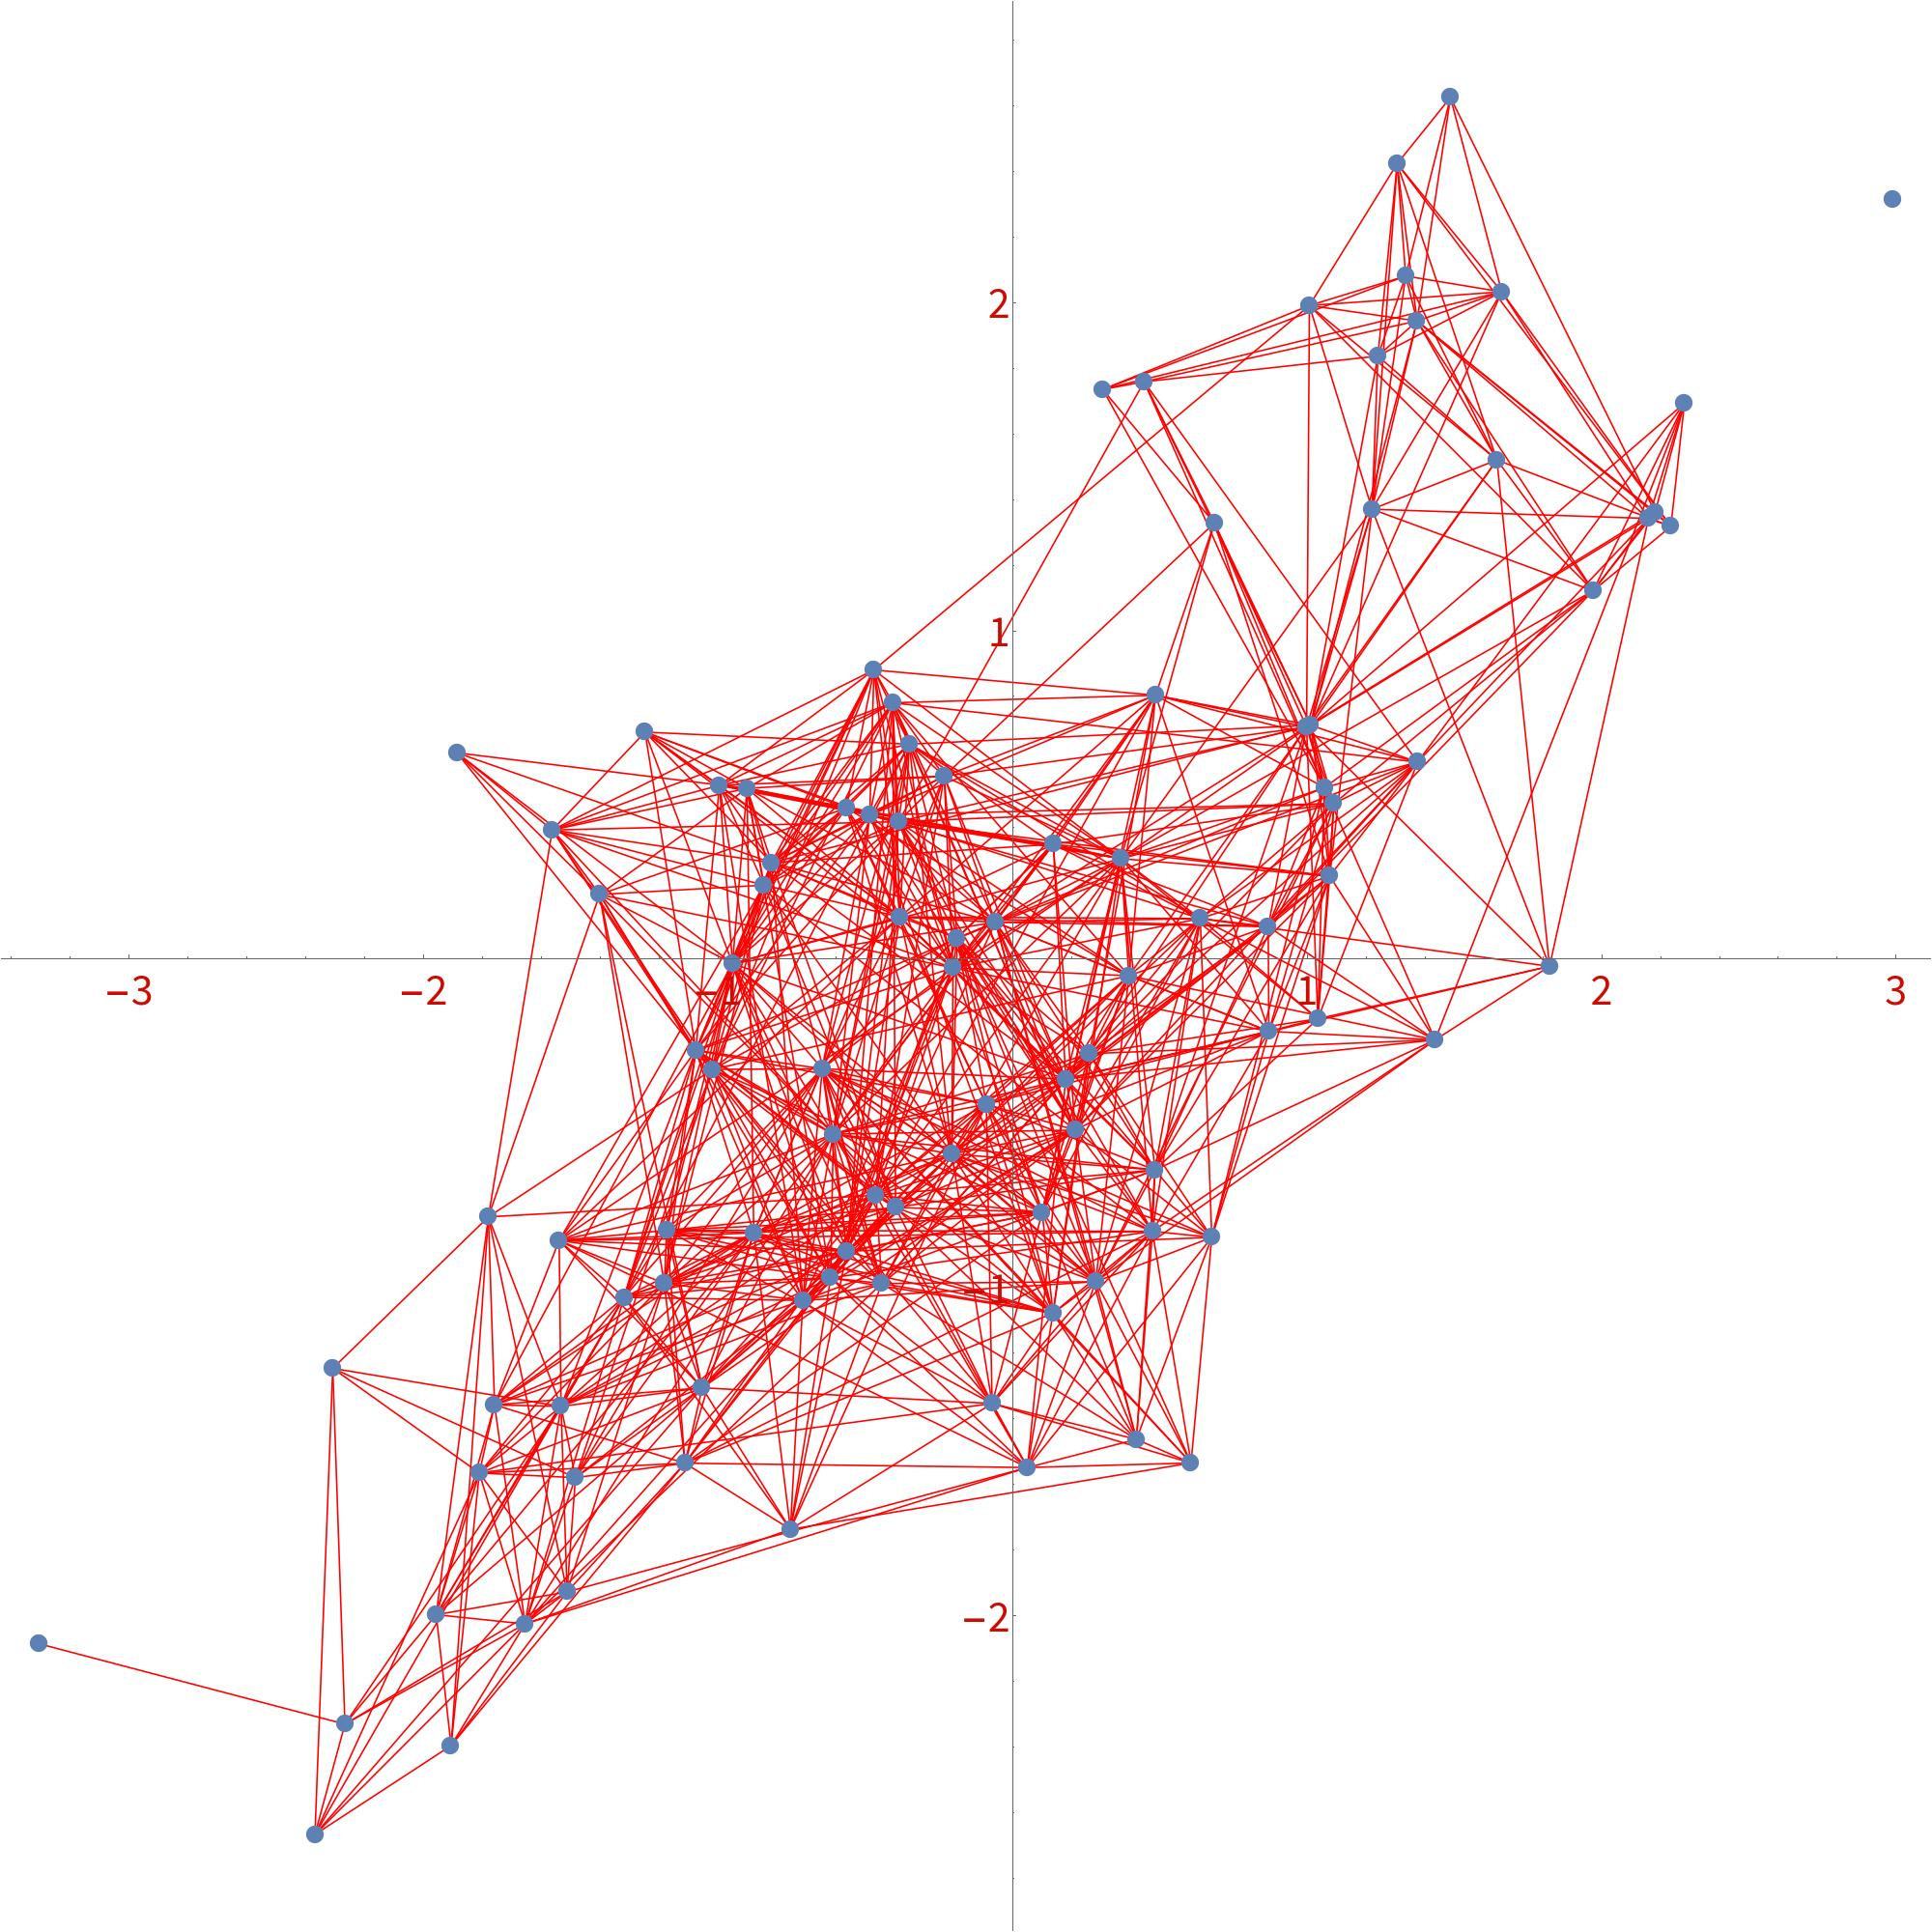
\includegraphics[width = 0.5\textwidth]{gaussian_rgg_non_spherical1.jpg}
    \caption[Gaussian non-spherical prior]{Gaussian prior with $\Sigma = \begin{pmatrix} 3 & 1.5 \\ 1.5 & 1\end{pmatrix}$}
    \label{fskewedg}
\end{subfigure}%
\begin{subfigure}{.5\textwidth}
    \centering
    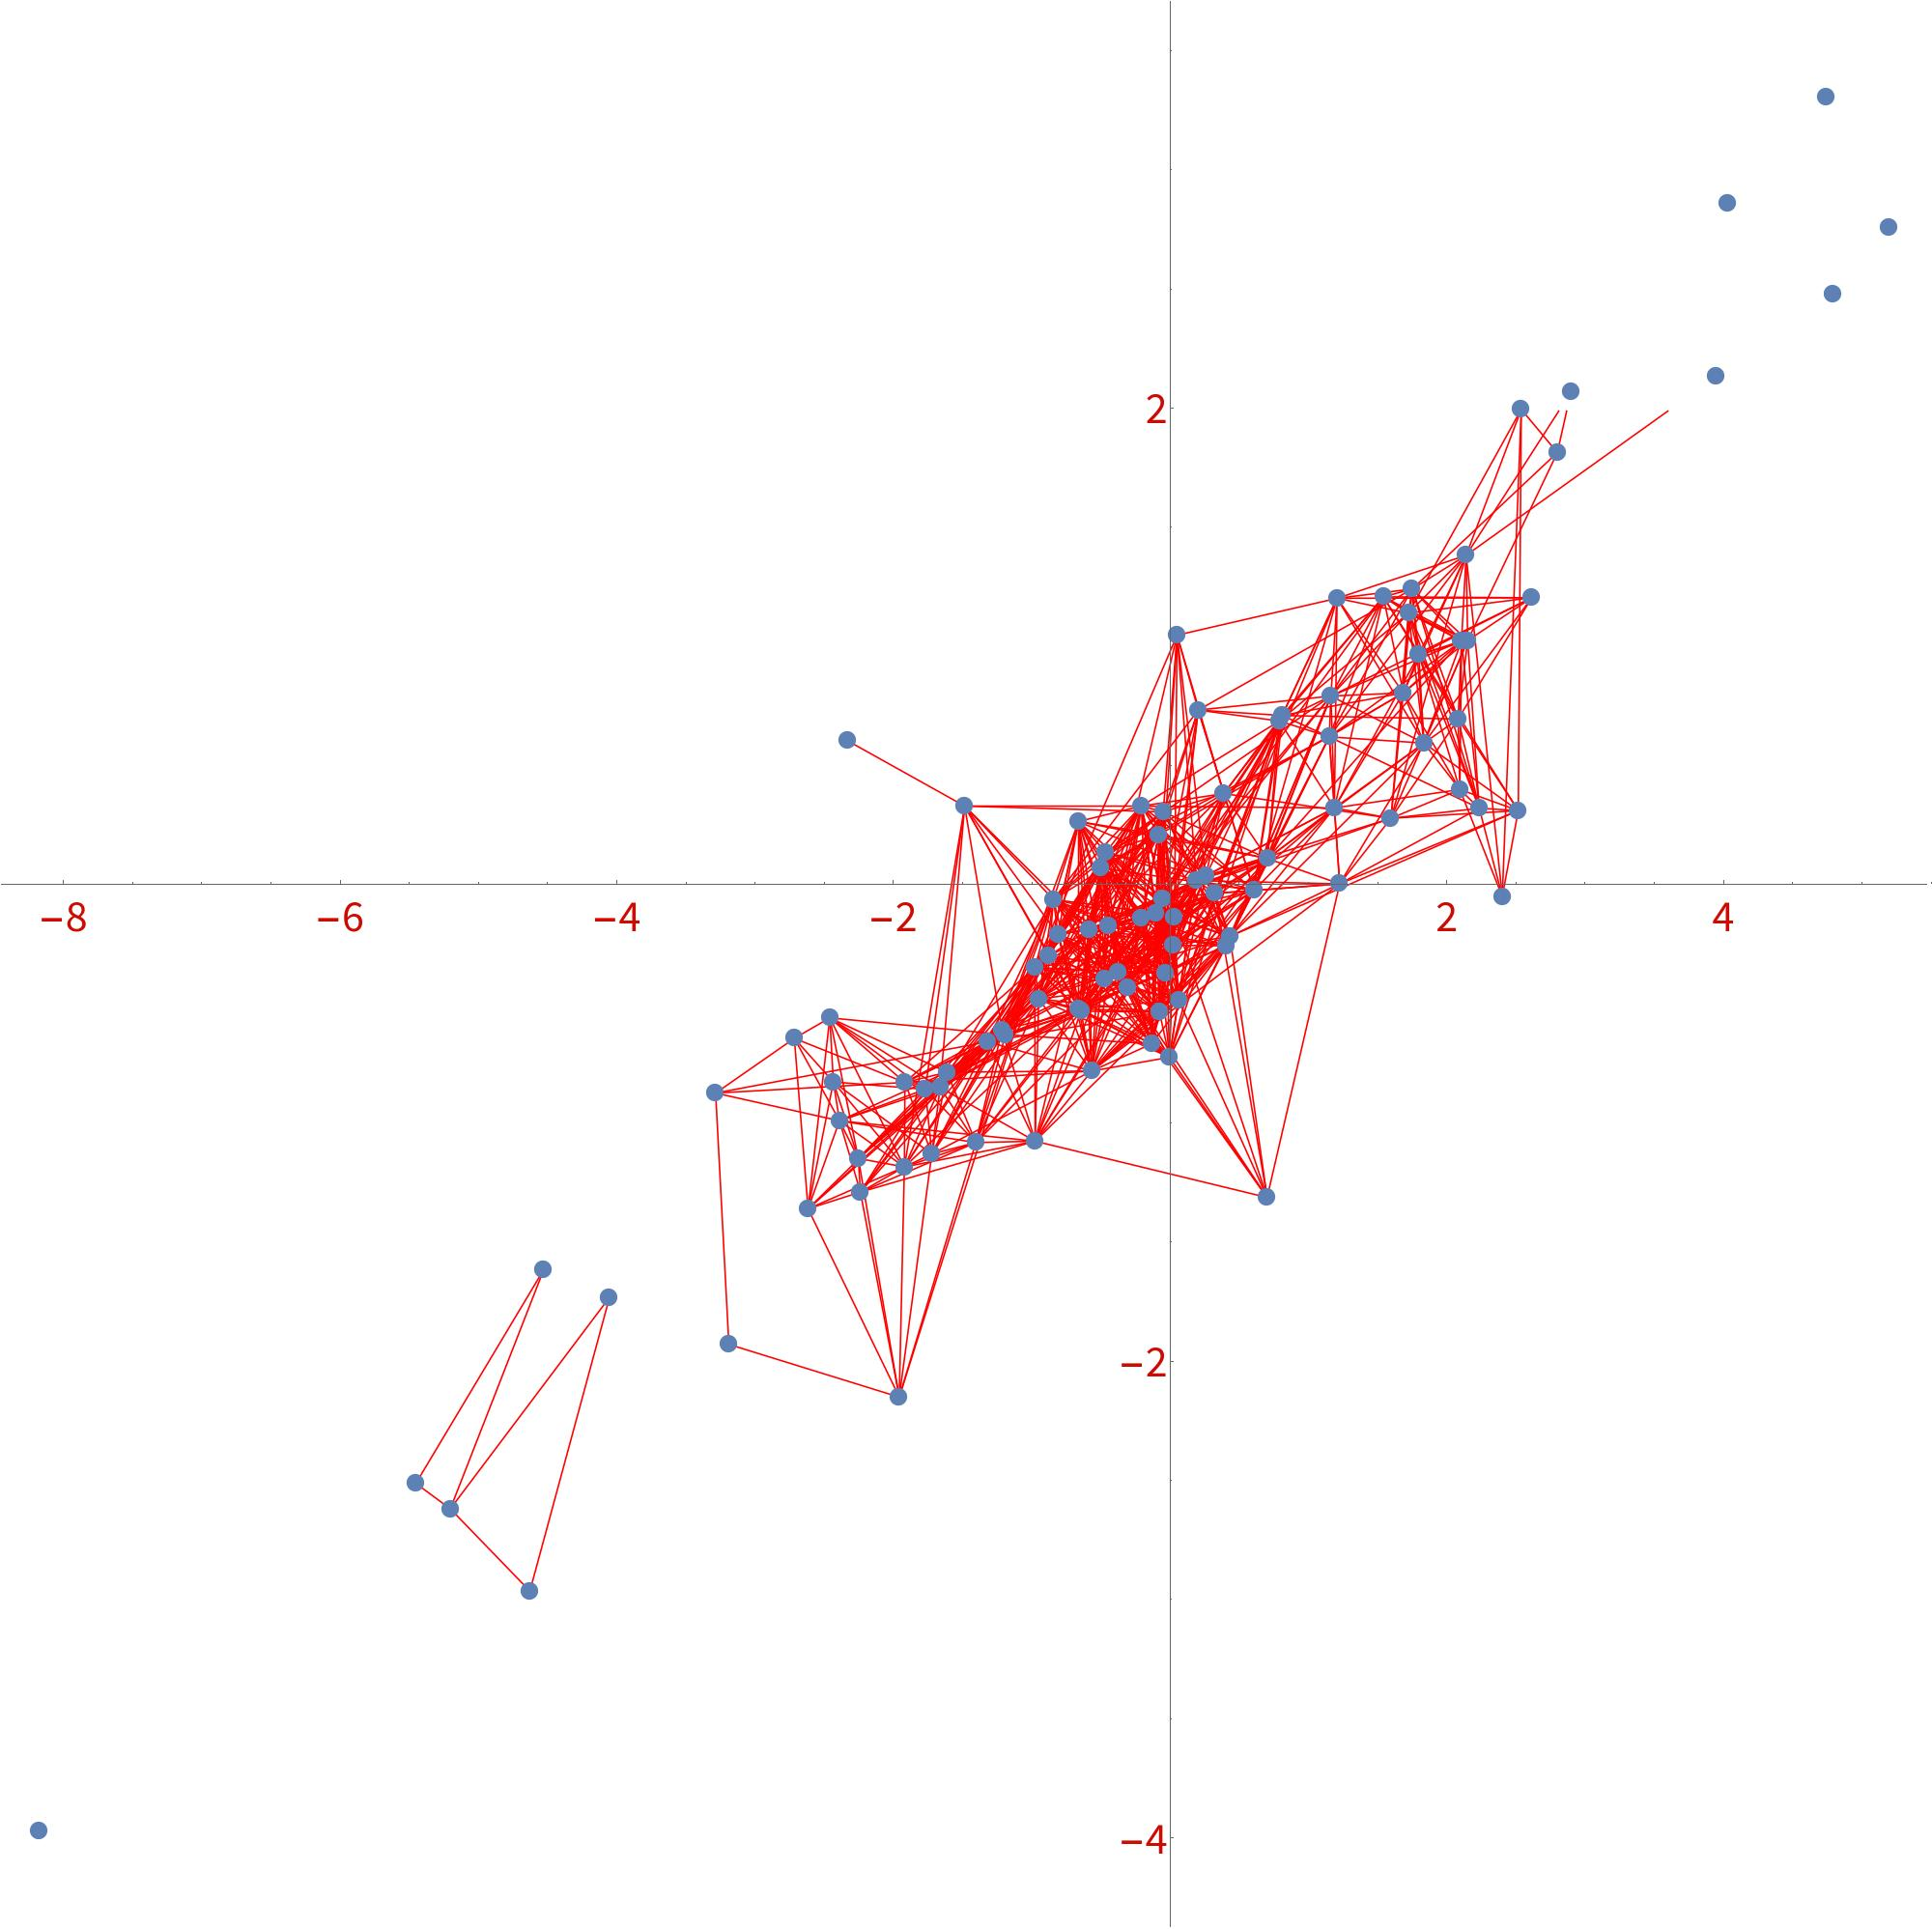
\includegraphics[width = 0.5\textwidth]{multivariatet_non_diag.jpg}
    \caption[Multivariate T]{Multivariate T with $\Sigma = \begin{pmatrix} 3 & 1.5 \\ 1.5 & 1\end{pmatrix}$ and 5 degrees of freedom.}
    \label{fskewedt}
\end{subfigure}
\end{figure}

So far we have only dealt with $2D$ data, so we ought to vary the number of dimensions as well. As we increase the number of dimensions $n$, the distances between points decrease, leading to a smaller number of edges. As a result, the largest total variation distances are for smaller $n$, since for larger $n$ more of the mass is concentrated around a smaller set in the distributions of the $d_k$, $\chi_k$ and $\gamma_k$ statistics. \\
\begin{table}[!ht]
    \centering
    \tiny
    \csvreader[tabular=lllllll,
        head=false,
        late after line=\\,
        late after first line=\\\midrule,
        table foot=\bottomrule,
        ]{test_ms.csv}{}{\csvcoli & \csvcolii & \csvcoliii & \csvcoliv & \csvcolv & \csvcolvi & \csvcolvii}
    \caption[Multiple ms]{Gaussian embeddings with identity covariance matrix for different values of $n$.}
\end{table}

The inferred $\sigma$ is generally underestimated, and, since the variance of the spherical Gaussian distribution we are using as the approximate distribution directly determines how spread out the embeddings are, hence the distances between pairs of them, the measured statistics expose subpar results. An obvious problem is the presence of the intractable integral, which leads to worse approximations as $\sigma$ increases. Another aspect that contributes to the poor results is the inflexible nature of the approximating distribution. The normal distribution is one of the easiest to work with, nevertheless, it still leads to intractable probability density functions for the squared distance between embeddings governed by it, unless we make it spherical. \\

\chapter{Summary and Conclusion}
In this thesis, we studied the potential of using random vertex embeddings as latent variables for a given adjacency matrix representing a graph, working in the framework of random geometric graphs. We investigated Euclidean, spherical and hyperbolic spaces and relied on Bayesian variational inference to approximate the posterior. \\

A possible extention of this model is approximating the posterior using a mixture of Gaussians. However, the probability density function of the squared distance between two random variables governed by different normal distributions has a closed form only if the two distributions share the mean, so not a lot of flexibility is provided by this. One can instead work with the distance as a random variable, instead of the squared distance, thus relying on noncentral $\chi^2$ distribution for the probability density function, although this introduces the modified Bessel function of the first kind which, combined with another intractable integral, might give rise to issues when approximating. \\

The most challenging aspect of this work was the form of the probability density function for the distance between pairs of embeddings, which forced us to make assumptions that severly limited our model. Even for something as simple as a spherical multivariate Gaussian prior, we run into an intractable integral and the right parameters are not recovered for simple data. It gets even more complicated when placing the embeddings on the unit sphere or in a hyperbolic space, with little hope of generating sensible results when considering the distances as random variables. \\

\appendix
\printbibliography


\chapter{Distance PDF}\label{appendix}
\raggedright

Let
\begin{equation*}
    X_i, X_j \sim \mathcal{N}(\bs{0}, \half\sigma^2\mc{I}_n)
\end{equation*}

Then
\begin{equation*}
    Y_{ij} = X_i - X_j \sim \mathcal{N}(\bs{0}, \sigma^2\mc{I}_n)
\end{equation*}

Denoting the squared distance between $X_i$ and $X_j$ by the random variable
\begin{equation*}
    D_{ij} = Y_{ij}^TY_{ij}
\end{equation*}
we find ourselves in the context defined in Mathai, so we have that the pdf of $D_{ij}$ is
\begin{equation*}
    f(u) = \sumlim{k}{0}{\infty}(-1)^kc_k\frac{u^{\frac{n}{2}+k-1}}{\Gamma(\frac{n}{2}+k)}
\end{equation*}
where
\begin{align}
    c_0 &= \prodlim{j}{1}{n}(2\lambda_j)^{-\half} \notag\\
    c_k &= \frac{1}{k}\sumlim{r}{0}{k-1}d_{k-r}c_r,\quad k\geq1 \\
    d_k &= \half\sumlim{j}{1}{n}(2\lambda_j)^{-k},\quad k\geq1 \notag
\end{align}
with $\{\lambda_j\}$ denoting the eigenvalues of the covariance matrix of $Y_{ij}$, $\sigma^2\mathcal{I}_n$, so
\begin{equation*}
    \lambda_j = \sigma^2,\quad j\in\{1,\,\dots,\,n\}
\end{equation*}
implying
\begin{align}
    c_0 &= (2\sigma^2)^{-\frac{n}{2}} \\
    d_k &= \half\sumlim{j}{1}{n}(2\sigma^2)^{-k} \notag\\
        &= \frac{n}{2}(2\sigma^2)^{-k},\quad k\geq1
\end{align}

Assuming that $n = 2m,\,m\in\mb{N}$, we will prove by induction that
\begin{equation*}
    c_k = \comb{m + k - 1}{k}2^{-k-m}(\sigma^2)^{-m - k},\quad k \geq 0
\end{equation*}
where $\comb{a}{b}$ denotes combinations of $a$ taken $b$. For the sake of the notation, let us assume that $\comb{0}{0} = 1$. \\

From (A.2), we have that
\begin{align*}
    c_0 &= 2^{-\frac{n}{2}}(\sigma^2)^{-frac{n}{2}} \\
    &= \ub{1}_{\comb{m-1}{0}} \times 2^{-m}(\sigma^2)^{-m}
\end{align*}
so the induction hypotesis holds for $c_0$. \\

Now, assuming that the hypothesis holds for $c_j,\,j\in\{0,\,\dots,\,k-1\}$, we will prove it holds for $c_k$ as well. Let us calculate each term of (A.1).

\begin{align*}
    d_{k-r}c_r &= m2^{-k+r}(\sigma^2)^{-k+r} \times \comb{m+r-1}{r}2^{-r-m}(\sigma^2)^{-m-r} \\
    &= m\comb{m+r-1}{r} 2^{-k-m}(\sigma^2)^{-k-m} 
\end{align*}
Then
\begin{align}
    c_k &= \frac{1}{k}\sumlim{r}{0}{k-1}m\comb{m+r-1}{r} 2^{-k-m}(\sigma^2)^{-k-m} \notag\\
    &= \frac{m}{k}2^{-k-m}(\sigma^2)^{-k-m}\sumlim{r}{0}{k-1}\comb{m+r-1}{r}  \\
\end{align}
We will prove by induction over k that $\sumlim{r}{0}{k-1}\comb{m+r-1}{r} = \comb{m+k-1}{k-1}$. For $k = 1$ it obviously holds. Assuming our assumption is true for some $k$, we will prove it holds for $k+1$ as well.
\begin{align*}
    \sumlim{r}{0}{k}\comb{m+r-1}{r} &= \sumlim{r}{0}{k-1}\comb{m+r-1}{r} + \comb{m+k-1}{k} \\
    &= \comb{m+k-1}{k-1} + \comb{m+k-1}{k} \\
    &= \comb{m+k}{k}
\end{align*}
making the induction proof complete.

(A.4) then becomes
\begin{align*}
    c_k &= \frac{m}{k}\comb{m+k-1}{k-1}2^{-k-m}(\sigma^2)^{-k-m} \\
    &= \comb{m+k-1}{k}2^{-k-m}(\sigma^2)^{-k-m}
\end{align*}
so the induction is complete. We now have that
\begin{align*}
    f(u) &= \sumlim{k}{0}{\infty}(-1)^k\comb{m+k-1}{k}2^{-k-m}(\sigma^2)^{-k-m}\frac{u^{m+k-1}}{\Gamma(m+k)} \\
    &= \sumlim{k}{0}{\infty}(-1)^k\frac{(m+k-1)!}{(m-1)!k!}2^{-k-m}(\sigma^2)^{-k-m}\frac{u^{m+k-1}}{(m+k-1)!} \\
    &= \sumlim{k}{0}{\infty}(-1)^k\frac{\cancel{(m+k-1)!}}{(m-1)!k!}2^{-k-m}(\sigma^2)^{-k-m}\frac{u^{m+k-1}}{\cancel{(m+k-1)!}} \\
    &= \frac{2^{-m}(\sigma^2)^{-m}u^{m-1}}{(m-1)!}\sumlim{k}{0}{\infty}(-1)^k\frac{1}{k!}2^{-k}(\sigma^2)^{-k}u^{k} \\
    &= \frac{2^{-m}(\sigma^2)^{-m}u^{m-1}}{(m-1)!}\sumlim{k}{0}{\infty}\frac{(-(2\sigma^2)^{-1}u)^k}{k!} \\
    &= \frac{(2\sigma^2)^{-m}u^{m-1}}{(m-1)!}e^{-(2\sigma^2)^{-1}u}
\end{align*}
\end{document}
